\chapter{Numerical Methods}
\label{ch:numerical_approx}

\section{Pricing Options via the Binomial Model}

Binomial pricing model arises from discrete random walk models of the underlying asset. The idea is to break down the time to expiration into potentially very large number ($N$) of time steps ($0, dt, 2dt,\ldots , ndt$ where $n\leq N$) . First step is to initialize the tree of stock prices by moving forward from today to expiration. At each step it is assumed that the stock price will move up (by the factor of $u$) or down (factor $d$).

One should find a way to calibrate the lattice so that it reflects the underlying model which is a continuous-time, continuous-state stochastic differential equation. Following this model, no-arbitrage and risk neutral principles crucial parameters are then obtained.

Risk-neutrality demands: $Se^{rdt} = pSu + (1-p)Sd$ that is $e^{rdt} = pu + (1-p)d$, where $p$ is the probability of an upward movement (and since we are dealing with a binomial tree $(1-p)$ is the probability of a downward movement). The previous equation reflects that discounted expected return equals current price.

\tikzstyle{bag} = [text width=2em, text centered]
\tikzstyle{end} = []
\begin{tikzpicture}[sloped]
	\node (a) at ( 0,0) [bag] {$\$ A$};
	\node (b) at ( 4,-1.5) [bag] {B};
	\node (c) at ( 4,1.5) [bag] {C};
	\node (d) at ( 8,-3) [bag] {D};
	\node (e) at ( 8,0) [bag] {E};
	\node (f) at ( 8,3) [bag] {F};
	\draw [->] (a) to node [below] {$(1-p)$} (b);
	\draw [->] (a) to node [above] {$P$} (c);
	\draw [->] (c) to node [below] {$P^2$} (f);
	\draw [->] (c) to node [above] {$(1-p)p$} (e);
	\draw [->] (b) to node [below] {$(1-p)p$} (e);
	\draw [->] (b) to node [above] {$(1-p)^2$} (d);
\end{tikzpicture}

Using condition introduced by Cox, Ross, Rubbenstein
\begin{equation}
u = \cfrac{1}{d}
\end{equation}

it can be obtained

\begin{equation}
\begin{gathered}
p=\cfrac{e^{rdt}-d}{u-d}\\
u = e^{\sigma\sqrt{dt}} \\
d = e^{-\sigma\sqrt{dt}}
\end{gathered}
\end{equation}
It can be concluded that tree recombines so that in every time step we have in $i^{th}$ step $i+1$ prices (some are recombined, $i=0\ldots N$), totaling $(N+1)(N+2)/2$ nodes (lattices) in trees of $N$ steps. Also there are $2N+1$ different possible price. Furthermore, as price at time zero is known ($S_0$), all feasible prices are obtained using
\begin{equation}
Su^j d^{i-j}\textrm{ or }Su^{2j-i}\textrm{, since }u=\cfrac{1}{d}
\end{equation}

Having the tree of stock prices constructed, and the option price can be derived working backward in the tree. %At the final step of the tree, i.e. at expiration of the option, the option values for each possible stock price are known, as they are equal to their intrinsic values. 
Assuming that the payoff function of the option is determined only by the value of the underlying asset at expiration, the model then works backwards through each time interval, calculating the option value at each step. The final step is at current time and stock price, where the theoretical fair value of the option is calculated. Algebraically it means for call option:
\begin{equation}
f_{N,j} = \textrm{max}(S_0 u^{j} d^{N-j} - K, 0),\quad j=0,1,\ldots , N
\end{equation}
\noindent
and for a put option
\begin{equation}
f_{N,j} = \textrm{max}(K - S_0 u^{j} d^{N-j}, 0),\quad j=0,1,\ldots , N
\end{equation}
Followed by working backward through the tree
\begin{equation}\
f_{i,j} = e^{-rdt}\left(pf_{i+1,j+1} + (1-p)f_{i+1,j}\right),\quad j=0,1,\ldots , i
\end{equation}
where $j$ denotes lattice position in $i^{th}$ step of the tree, so it can take values up to $i$.

The main reason for introducing Binomial trees was inability to calculate the price of an American style option using Black-Scholes equation. With Binomial trees it is straightforward to take into account early exercise possibility in American calls and puts:
\begin{equation}
\begin{gathered}
f_{i,j} = \textrm{max}\left(S_0 u^{j} d^{N-j} - K, e^{-rdt}\left(pf_{i+1,j+1} + (1-p)f_{i+1,j}\right)\right) \\
f_{i,j} = \textrm{max}\left(K - S_0 u^{j} d^{N-j}, e^{-rdt}\left(pf_{i+1,j+1} + (1-p)f_{i+1,j}\right)\right)
\end{gathered}
\end{equation}

Below the \texttt{python} code to generate binomial trees for European and American options.
The example computes using a 5-steps binomial tree the price of an European call with $r=0.1, \sigma=0.4, T=1, S_0=50, K=50$.

\begin{ipython}
import math

class Node:
    def __init__(self, i, j, S0, u, K, iscall):
        self.i = i
        self.j = j
        self.S = S0*u**(2*j-i)
        if iscall:
            self.P = max(self.S - K, 0)
        else:
            self.P = max(K - self.S, 0)
        
class Tree:
    def __init__(self, r, sigma, N, T, S0, K, iscall = True, isamerican = False):
        self.iscall = iscall
        self.isamerican = isamerican
        self.S0 = S0
        self.K = K
        self.r = r
        self.sigma = sigma
        self.N = N + 1
        self.dt = T/N
        self.u = math.exp(self.sigma*math.sqrt(self.dt))
        self.d = 1/self.u
        self.p = (math.exp(self.r*self.dt)-self.d)/(self.u - self.d)
        self.nodes = []
        for i in range(self.N):
            tmp = []
            for j in range(i+1):
                node = Node(i, j, self.S0, self.u, self.K, self.iscall)
                tmp.append(node)
            self.nodes.append(tmp)
            
    def price(self):
        for i in range(len(self.nodes)-2, -1, -1):
            nds = self.nodes[i]
            for j in range(len(nds)):
                nds[j].P = math.exp(-self.r*self.dt)* \
                                (self.p*self.nodes[i+1][j+1].P + \
                                (1-self.p)*self.nodes[i+1][j].P)
                if self.isamerican:
                    S = self.S0*self.u**(2*j-i)
                    if self.iscall:
                        exercise = max(S - self.K, 0)
                    else:
                        exercise = max(self.K - S, 0)

                    nds[j].P = max(nds[j].P, exercise)
        return self.nodes[0][0].P
            
    def print(self):
        for layer in myTree.nodes:
            for n in reversed(layer):
                print ("{:8.4f} {:8.4f}".format(n.S, n.P)) 
            print ("")

myTree = Tree(0.1, 0.4, step, 1, 50, 50, True, False)    
print ("Options price: {:.4f}".format(myTree.price()))
myTree.print()
\end{ipython}
\begin{ioutput}
Options price: 10.4968
 50.0000  10.4968

 59.7942  16.5321
 41.8101   4.6099

 71.5069  25.3174
 50.0000   8.0145
 34.9617   1.2348

 85.5139  37.4745
 59.7942  13.6320
 41.8101   2.4626
 29.2350   0.0000

102.2647  53.2548
 71.5069  22.4970
 50.0000   4.9111
 34.9617   0.0000
 24.4464   0.0000

122.2967  72.2967
 85.5139  35.5139
 59.7942   9.7942
 41.8101   0.0000
 29.2350   0.0000
 20.4421   0.000
\end{ioutput}

Figure~\ref{fig:binomial_tree_accuracy} shows how the accuracy of the Binomial tree technique improves with the number of steps.
It can be noticed that binomial tree is not so good at the beginning (small number of steps used), but it converges to the right price every few steps. 

\begin{figure}[htb]
	\centering
	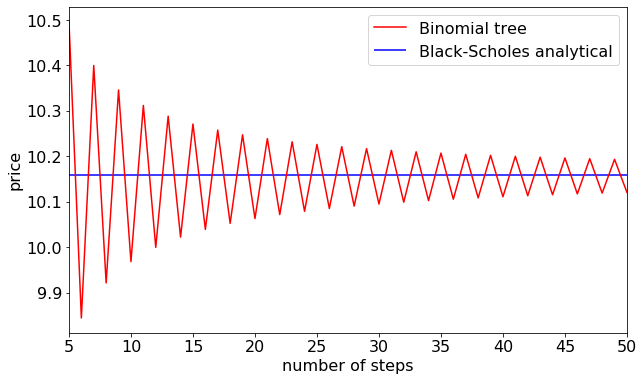
\includegraphics[width=0.7\textwidth]{figures/binomial_tree_accuracy}
	\caption{Accuracy of the Binomial tree technique as a function of the number of steps. The analytical price computed using Black-Scholes model is reported for comparison too.}
	\label{fig:binomial_tree_accuracy}
\end{figure} 
%Finite difference schemes are very much similar to trinomial tree options pricing, where each node is dependent on three other nodes with an up movement, a down movement, and a flat movement.

\section{Finite Differences} 
\label{sec:finite_difference}
A common method to numerically solve Ordinary Differential Equations (ODE), like heat equation, Black-Scholes equation, etc\ldots is the \emph{finite difference method}. An ODE is a differential equation containing one or more functions of one independent variable and the derivatives of those functions~\cite{bib:ode}. The term ordinary is used in contrast with the term partial differential equation (PDE) which may be with respect to more than one independent variable.
With this technique a differential equation is transformed into a system of algebraic equations to solve by approximating each derivative with finite difference formulas at evenly spaced grid points.

Imagine to divide the ranges $[0, S_max]$ and $[0, T]$ into $M$ and $N$ intervals respectively as shown in Figure~\ref{fig:finite_difference_1} (e.g. $S = i\Delta S$ with $i\in[0, M]$, $t = j\Delta t$ with $j \in[0,N]$).

The differential equation is enforced only at the grid points, and the first and second derivatives can be obtained as follows.
With the help of Taylor expansion indeed, we can discretize the derivatives in the ODE ($y(x, t)$) leading to a recursive formula for $y_{i,j}$ (assume $y\in\mathbb{C}^{n+1}$ and the grid spacing is small). For a point $x_i$ between $x$ and $x+h$,

\begin{equation}
y(x+h)=y(x)+hy'(x)+\cfrac{1}{2}h^2y''(x)+\ldots+\cfrac{h^n}{n!}y^{(n)}(x)+\cfrac{h^{n+1}}{(n+1)!}y^{(n+1)}(ξ)
\end{equation}

Replacing terms after $h^2$ with $O(h^2)$ and moving $y'(x)=\cfrac{\partial y}{\partial x}$ to the left-hand side, we have the \emph{forward difference}, which has error order 1

\begin{equation}
%\begin{split}
y(x+h)=y(x)+hy'(x)+\cfrac{1}{2}h^2y''(x)+O(h^2)
\implies \cfrac{\partial y}{\partial x} = \cfrac{y(x+h)−y(x)}{2h}
%\end{split}
\end{equation}

Likewise, $y'$ and $y''$ can be approximated by \emph{backward difference} and \emph{central difference}. Figure~\ref{fig:graph_finite_difference} shows a graphical representation of the different types of finite differences. Commonly, the central difference formulas is used, due to the fact that it yields better accuracy. 
Table~\ref{tab:derivative_approximations} reports a summary of derivatives approximation.

\begin{figure}[htb]
	\centering
	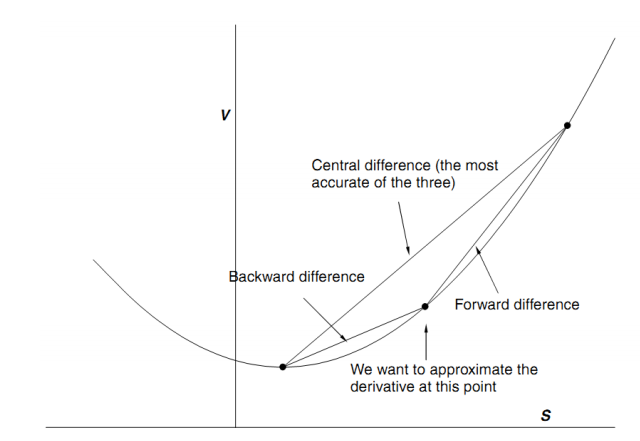
\includegraphics[width=0.7\textwidth]{figures/graph_finite_difference}
	\caption{Graphical representation of first order derivative using backward, forward and central difference.}
	\label{fig:graph_finite_difference}
\end{figure} 
 
\begin{table}[htb]
    \centering
    \begin{tabular}{|l|c|c|}
    \hline
    Type & Approximation & Error Order \\
    \hline
    Forward difference & $\cfrac{\partial y}{\partial x} = \cfrac{y_{i+1,j}-y_{i,j}}{\Delta x}$, $\cfrac{\partial y}{\partial t} = \cfrac{y_{i,j+1}-y_{i,j}}{\Delta x}$ & 1 \\[1ex]
    \hline
    Backward difference & $\cfrac{\partial y}{\partial x} = \cfrac{y_{i,j}-y_{i-1,j}}{\Delta x}$ & 1 \\[1ex]
    \hline
    Central difference & $\cfrac{\partial y}{\partial x} = \cfrac{y_{i+1,j}-y_{i-1,j}}{2\Delta x}$& 2 \\[1ex]
    \hline
    Second difference & $\cfrac{\partial^2 y}{\partial x^2} = \cfrac{y_{i+1,j}-2y_{i,j} + y_{i-1,j}}{\Delta x^2}$& 2 \\[1ex]
    \hline
    \end{tabular}
\caption{Summary of derivative approximations and relative errors.}
\label{tab:derivative_approximations}
\end{table}

These finite difference expressions are used to replace the derivatives of $y$ in the differential equation which leads to a system of $n+1$ linear algebraic equations if the differential equation is linear. If the differential equation is nonlinear, the algebraic equations will also be nonlinear.

Depending on which combination of presented schemes for derivatives is used in the discretization of the equation, one can end up with different approaches, \emph{explicit}, \emph{implicit} or \emph{Crank-Nicolson}. Graphical illustration of these methods are shown with the grid in Fig.~\ref{fig:grid_finite_difference}. 
Table ~\ref{tab:various_methods} summarizes the possibilities.

\begin{figure}[htb]
	\centering
	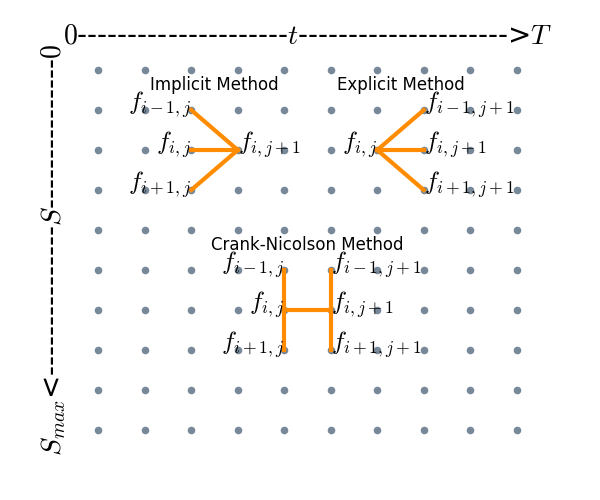
\includegraphics[width=0.7\textwidth]{figures/grid_finite_differences}
	\caption{Example of grid used to solve an Ordinary Differential Equation.}
	\label{fig:grid_finite_difference}
\end{figure} 

\begin{table}[htb]
    \centering
    \begin{tabular}{|l|c|c|}
    \hline
    Method & x-derivatives & time-derivatives \\
    \hline
    Explicit & central difference & backward difference \\
    \hline
    Implicit & central difference & forward difference \\
    \hline
    Crank-Nicolson & central difference & central difference \\
    \hline
    \end{tabular}
\caption{Possible variations of finite difference method.}
\label{tab:various_methods}
\end{table}

\subsection{Boundary Conditions}
Before delving into some example applications, we need to discuss the choice of boundary conditions which is an important issue in the construction of these methods. Well chosen boundary conditions contribute to preventing any errors on the boundaries propagated through the rest of the mesh. There are several ways to specify boundary conditions the most common are:

\begin{itemize}
\item Dirichlet Condition: a Dirichlet boundary condition assigns a value to $y$ at boundary. For example, imagine to price a call option with the finite difference method. At $S_{min}=0$, the option value could be set to zero, since the it is worthless. However, if underlying price reaches $S_{max}$ at time $t$, the option is worth the discounted value of its expected payoff. For a vanilla call option:

\begin{equation*}
\begin{cases}
y(0,t)=0(4)\\
y(S_{max},t)=S_{max}−Ke^{−r(T−t)}
\end{cases}
\end{equation*}
\item Neumann Condition: Neumann condition specifies the partial derivative at the boundary. Discretizing the second derivative at the boundary by central difference gives us a more friendly equation about $y_{i,j}$. In addition, the Neumann condition is inclined to be more accurate for the same boundaries than the Dirichlet conditions.
\begin{equation*}
\begin{cases}
\cfrac{\partial^2 f}{\partial x^2}(\Delta x,t)=0 \implies y_{0,j}−2y_{1,j}+y_{2,j}=0\\[1ex]
\cfrac{\partial^2 f}{\partial x^2}((N−1)\Delta x,t) =0\implies y_{M−2,j}−2y_{M−1,j}+y_{M,j}=0
\end{cases}
\end{equation*}
\end{itemize}

%\subsection{Finite Difference Methods}
%In this section, we discretize the B-S PDE using explicit method, implicit method and Crank-Nicolson method and construct the matrix form of the recursive formula to price the European options. 

\subsection{Instabilities}
When discussing effectiveness of different finite difference methods, we should consider three fundamental properties, which are consistency, stability, and convergence. Furthermore, we have to notice that though numerical method is good for solving PDE, it also brings the truncation error due to the discretization of the variables (e.g. stock price and time).

\begin{itemize}
\item stability: a finite difference scheme is said to be stable if the difference between numerical solution and the true solution doesn't grow infinitely as the grid spacing approaches zero; %The stability of numerical scheme is achieved if the spectral radius of A less than 1.
\item consistency: a finite difference scheme is consistent if the difference between PDE and finite differential equation vanishes as the grid spacing approaches zero. That is, the truncation error tends to 0 as the mesh get infinitely finer.
\item convergence: a finite difference scheme is said to be convergent if solutions derived from a finite difference equation converge point-wise to the true solutions of the original PDE as the grid spacing approaches zero.
\end{itemize}

More quantitative statement concerning stability will be presented in the next Section in the context of the heat equation.

%\subsection{A Simple Application}
%Imagine we are going out to launch a rocket, and let $y(t)$ be the altitude (meters from the surface) of the rocket at time $t$. We know the gravity $g=9.8$~m/s$^2$. If we want to have the rocket at $50$~m off the ground after 5 seconds after launching, what should be the velocity at launching? 
%The ODE we need to solve is 
%
%\begin{equation*}
%\cfrac{\partial^2y}{\partial t^2} = -g
%\end{equation*}
%
%with the boundary conditions $y(0)=0$ and $y(5)=50$. Let’s take $n=10$, so let's make a grid with ten steps in time.
%
%Since the time interval is $[0,5]$ and we have chosen $n=10$, $h=0.5$, using the finite difference approximated derivatives, we have
%
%\begin{gather*}
%y0=0 \\
%y_{i−1}−2y_i+y_{i+1}=−gh^2,i=1,2,...,n−1\\
%y_{10}=50
%\end{gather*}
%
%If we use matrix notation, we will have:
%\begin{equation*}
%\begin{bmatrix}
%1 & 0\\
%1 & -2 & 1 \\
%  &  \ddots & \ddots & \ddots & \\
%  & &  1 & -2 & 1 \\
%  &  &  &  & 1 
%\end{bmatrix}
%\begin{bmatrix}
%y_0 \\
%y_1 \\
%\vdots \\
%y_{n-1} \\
%y_n 
%\end{bmatrix}
%=
%\begin{bmatrix}
%0\\
%-gh^2 \\
%\vdots \\
%-gh^2 \\
%50
%\end{bmatrix}
%\end{equation*}
%
%Therefore, we have 11 equations in the system, that can be solved using the method explained in Chapter~\ref{matrix-equations}.
%
%\begin{ipython}
%import numpy as np
%import matplotlib.pyplot as plt
%
%n = 10
%h = (5-0) / n
%
%# Get A
%A = np.zeros((n+1, n+1))
%A[0, 0] = 1
%A[n, n] = 1
%for i in range(1, n):
%    A[i, i-1] = 1
%    A[i, i] = -2
%    A[i, i+1] = 1
%
%print(A)
%
%# Get b
%b = np.zeros(n+1)
%b[1:-1] = -9.8*h**2
%b[-1] = 50
%print(b)
%
%# solve the linear equations
%y = np.linalg.solve(A, b)
%
%t = np.linspace(0, 5, 11)
%
%plt.figure(figsize=(10,8))
%plt.plot(t, y)
%plt.plot(5, 50, 'ro')
%plt.xlabel('time (s)')
%plt.ylabel('altitude (m)')
%plt.show()
%\end{ipython}
%\begin{ioutput}
%[[ 1.  0.  0.  0.  0.  0.  0.  0.  0.  0.  0.]
% [ 1. -2.  1.  0.  0.  0.  0.  0.  0.  0.  0.]
% [ 0.  1. -2.  1.  0.  0.  0.  0.  0.  0.  0.]
% [ 0.  0.  1. -2.  1.  0.  0.  0.  0.  0.  0.]
% [ 0.  0.  0.  1. -2.  1.  0.  0.  0.  0.  0.]
% [ 0.  0.  0.  0.  1. -2.  1.  0.  0.  0.  0.]
% [ 0.  0.  0.  0.  0.  1. -2.  1.  0.  0.  0.]
% [ 0.  0.  0.  0.  0.  0.  1. -2.  1.  0.  0.]
% [ 0.  0.  0.  0.  0.  0.  0.  1. -2.  1.  0.]
% [ 0.  0.  0.  0.  0.  0.  0.  0.  1. -2.  1.]
% [ 0.  0.  0.  0.  0.  0.  0.  0.  0.  0.  1.]]
%[ 0.   -2.45 -2.45 -2.45 -2.45 -2.45 -2.45 -2.45 -2.45 -2.45 50.  ]
%\end{ioutput}
%
%\begin{figure}[htb]
%	\centering
%	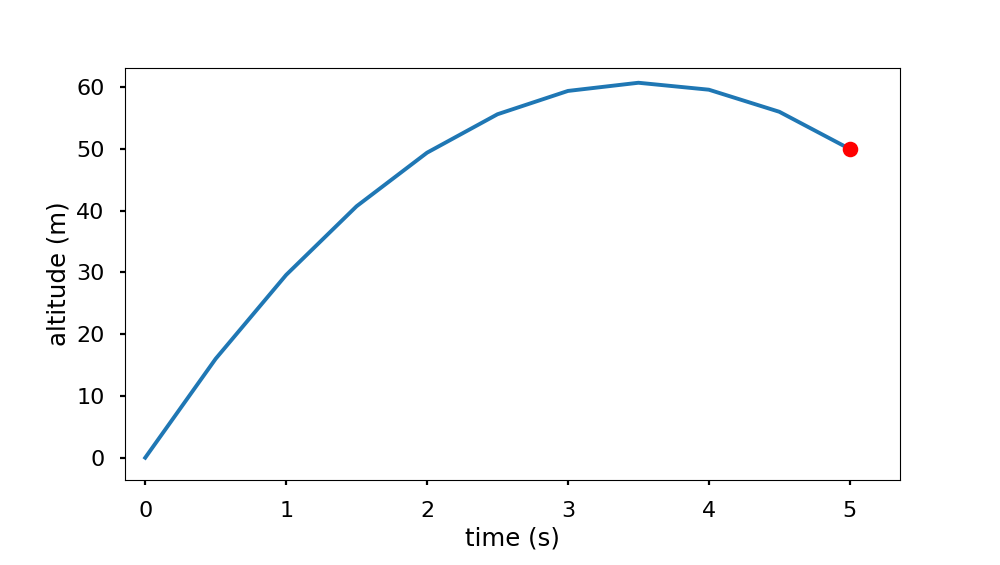
\includegraphics[width=0.9\textwidth]{figures/finite_difference}
%	\caption{Example of linear regression for the determination of $\beta$.}
%	\label{fig:finite_difference}
%\end{figure} 
%
%Now, let’s solve for $y'(0)$ in order to determine the intial velocity of the rocket. From the finite difference formula, we know that $\frac{dy}{dx}=\frac{y_{i+1}−y_{i−1}}{2h}$, which means that $y'(0)=\frac{y_1−y_{−1}}{2h}$, but we don’t know what is $y_{−1}$. Actually, we can calculate $y_{−1}$ since we know the $y$ values on each grid point. From the 2$^{nd}$ derivative finite difference formula, we know that $\frac{y_{−1}−2y_0+y_1}{h^2}=−g$, therefore, we can solve for $y_{−1}$ and then get the launching velocity. See the calculation below.
%
%\begin{ipython}
%y_n1 = -9.8*h**2 + 2*y[0] - y[1]
%(y[1] - y_n1) / (2*h)
%\end{ipython}
%\begin{ioutput}
%34.5
%\end{ioutput}

\section{2D Heat Equation}
Heat equation is a partial differential equation, defined as
\begin{equation}
\cfrac{\partial u}{\partial t} - \alpha\nabla u = 0
\end{equation}
\noindent 
It represents an important example since the Black-Scholes equation, through appropriate variable transformations, can be put in the same form. So learning to solve it helps in understanding the BS model.

Consider the the two-dimensionsal case, expliciting nabla the heat equation becomes
\begin{equation}
\cfrac{\partial u}{\partial t} - \alpha\left(\cfrac{\partial^2 u}{\partial x^2}+\cfrac{\partial^2 u}{\partial y^2}\right)= 0
\end{equation}
\noindent
where $t$ is for temporal variable, $x$ and $y$ are spatial variables, and $\alpha$ is the diffusivity constant. So basically we want to find the solution $u(\mathbf{x}, t)$ everywhere in $x$ and $y$, and over time $t$.

In order to get an approximate solution of the heat equation we are going to apply the finite difference method outlined in the previous Section. The first step is to "discretize" the spatial domain $x, y$ and the time interval $t$ like this

\begin{gather}
x_i = i\Delta x \\
y_i = j\Delta y \\
t_i = k\Delta t 
\end{gather}

As we can see, $i, j$, and $k$ represent the steps for each difference for $x, y,$ and $t$ respectively. What we want is the solution $u$, which is

\begin{equation}
u(x, y, t) = u_{i,j}^k
\end{equation}

We can write the heat equation above using the \emph{explicit} finite difference method like this

\begin{equation}
\cfrac{u_{i,j}^{k+1}-u_{i,j}^k}{\Delta t} - \alpha\left(\cfrac{u_{i+1,j}^{k}-2u_{i,j}^{k}+u_{i-1,j}^{k}}{\Delta x^2}+\cfrac{u_{i,j+1}^{k}-2u_{i,j}^{k}+u_{i,j-1}^{k}}{\Delta y^2}\right)=0
\end{equation}

If we arrange the equation above by taking $\Delta x = \Delta y$, we get the final equation

\begin{equation}
u_{i,j}^{k+1} = \gamma \left(u_{i+1,j}^{k}+u_{i-1,j}^{k}+u_{i,j+1}^{k}+u_{i,j-1}^{k}-4u_{i,j}^{k}\right)+u_{i,j}^{k}
\end{equation}
\noindent 
where
\begin{equation}
\gamma = \alpha\cfrac{\Delta t}{\Delta x^2}
\end{equation}

Now we can solve the heat equation approximated by the algebraic equation above, which is computer-friendly. As an example problem let’s suppose a thin square plate with the side of 50 unit length. The temperature everywhere inside the plate is originally (at $t = 0$) at 0 degree, see Figure~\ref{fig:heat_start_1}.

\begin{figure}[htb]
	\centering
	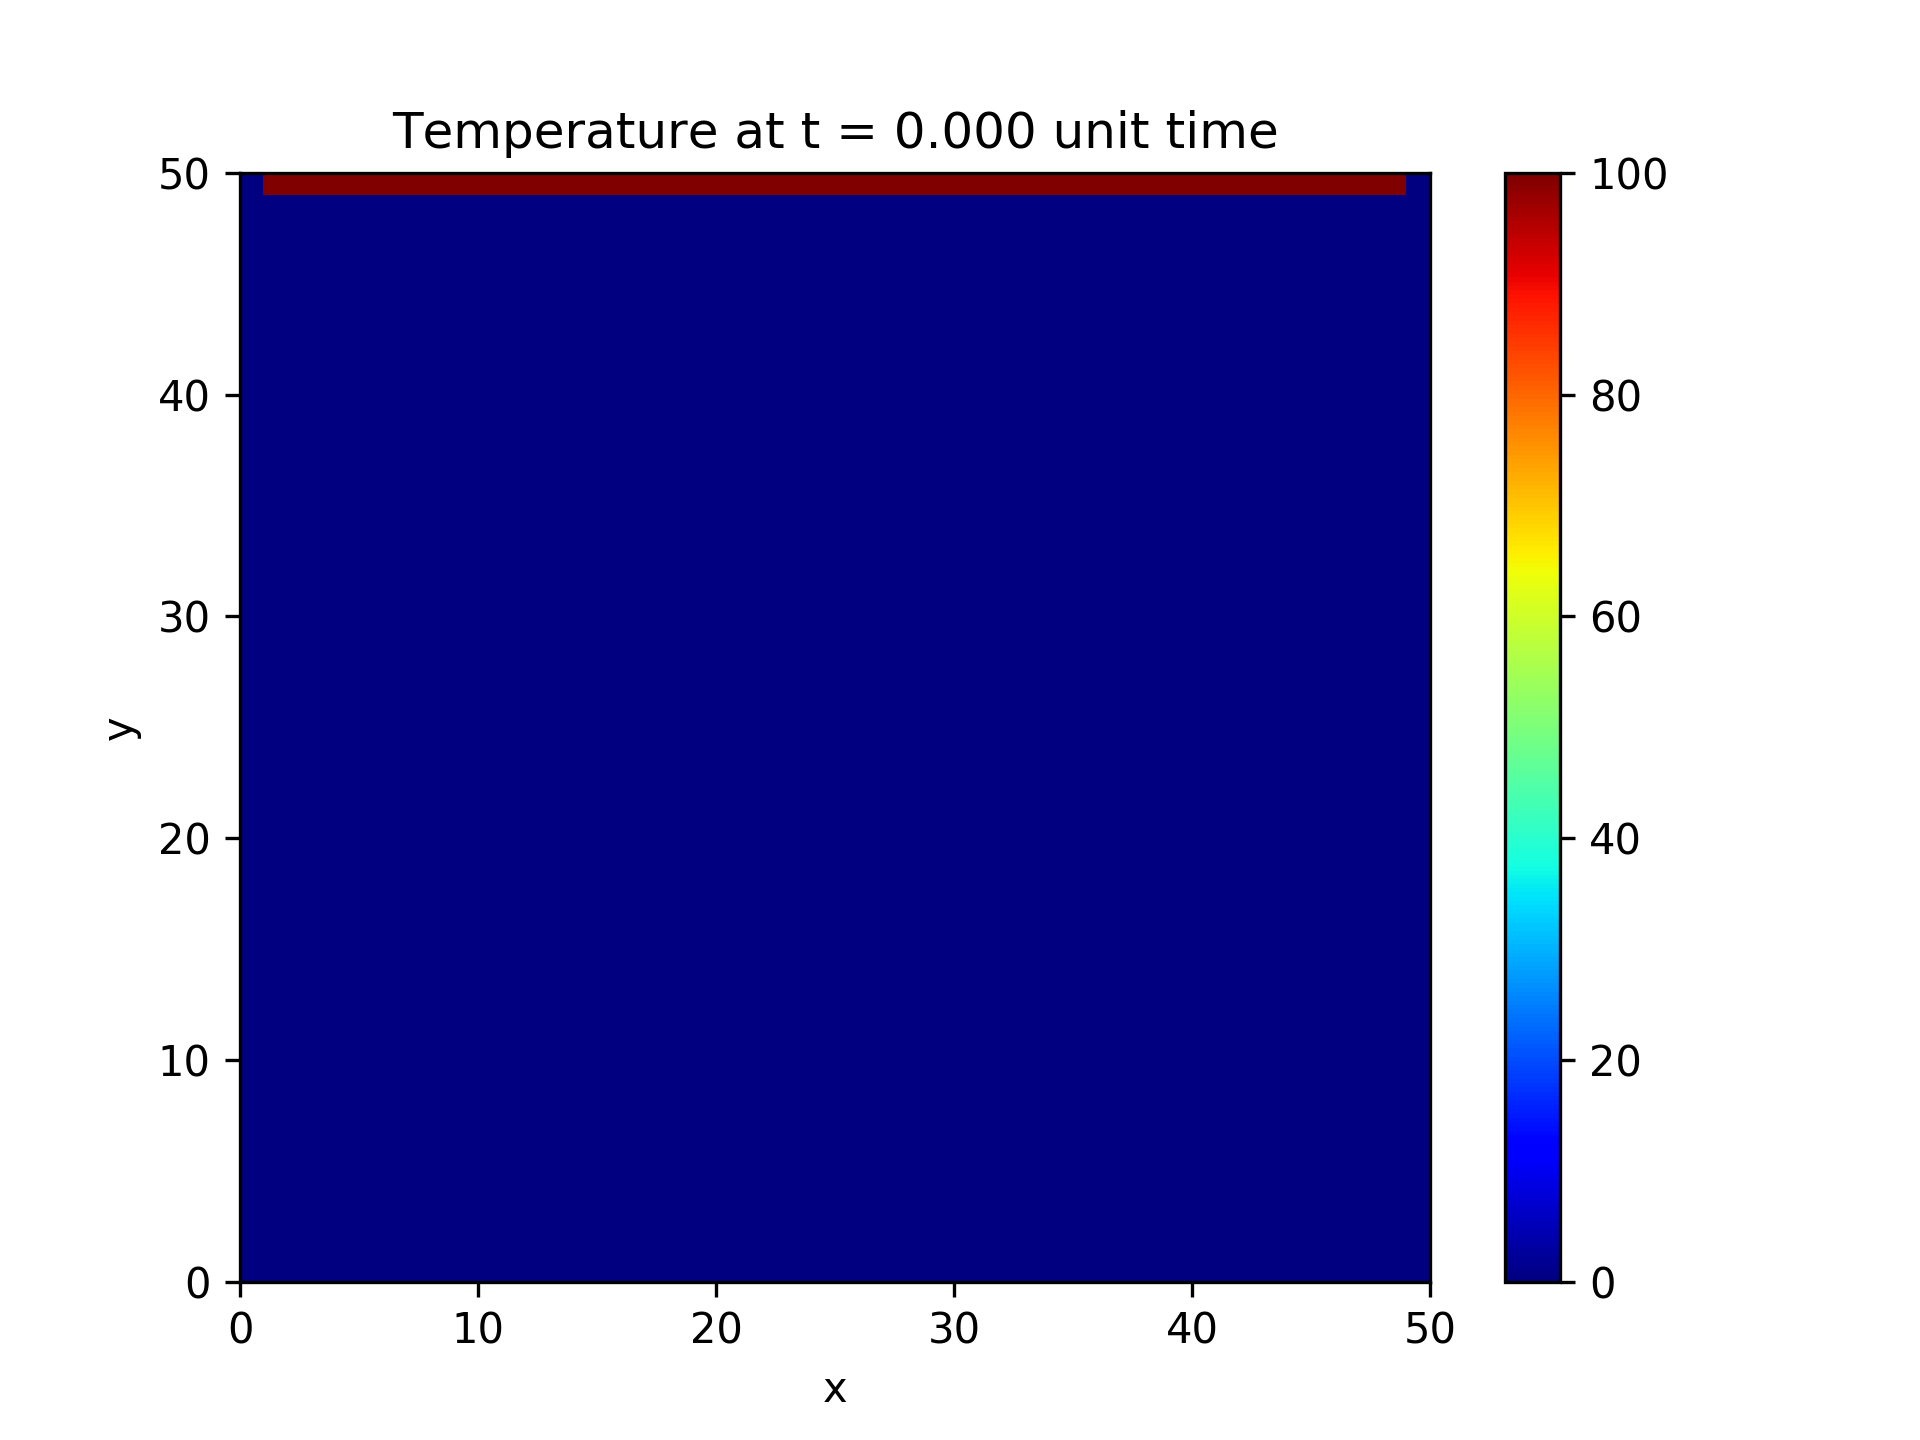
\includegraphics[width=0.7\textwidth]{figures/frame0}
	\caption{Boundary and initial conditions for our exercise.}
	\label{fig:heat_start_1}
\end{figure} 
\noindent
Let’s take $\Delta x = 1$ and $\alpha = 2.0$. Now we can write some \texttt{python} code to solve this problem numerically to see the temperature everywhere as a function of time. 

\begin{ipython}
import numpy as np

plate_length = 50
max_iter_time = 750

alpha = 2
delta_x = 1

delta_t = (delta_x ** 2)/(4 * alpha)
gamma = (alpha * delta_t) / (delta_x ** 2)

# Initialize solution: the grid of u(k, i, j)
u = np.empty((max_iter_time, plate_length, plate_length))

# Initial condition everywhere inside the grid
u_initial = 0

# Boundary conditions
u_top = 100.0
u_left = 0.0
u_bottom = 0.0
u_right = 0.0

# Set the initial condition
u.fill(u_initial)

# Set the boundary conditions
u[:, (plate_length-1):, :] = u_top
u[:, :, :1] = u_left
u[:, :1, 1:] = u_bottom
u[:, :, (plate_length-1):] = u_right

def calculate(u):
    for k in range(0, max_iter_time-1, 1):
        for i in range(1, plate_length-1, delta_x):
            for j in range(1, plate_length-1, delta_x):
                u[k + 1, i, j] = gamma * (u[k][i+1][j] + u[k][i-1][j] + 
                                          u[k][i][j+1] + u[k][i][j-1] - 
                                          4*u[k][i][j]) + u[k][i][j]

    return u

u = calculate(u)
\end{ipython}

Figure~\ref{fig:heat_end_1} shows the heat distribution after 62.5 seconds. The central part of the plate is now much warmer. 
\begin{figure}[htb]
	\centering
	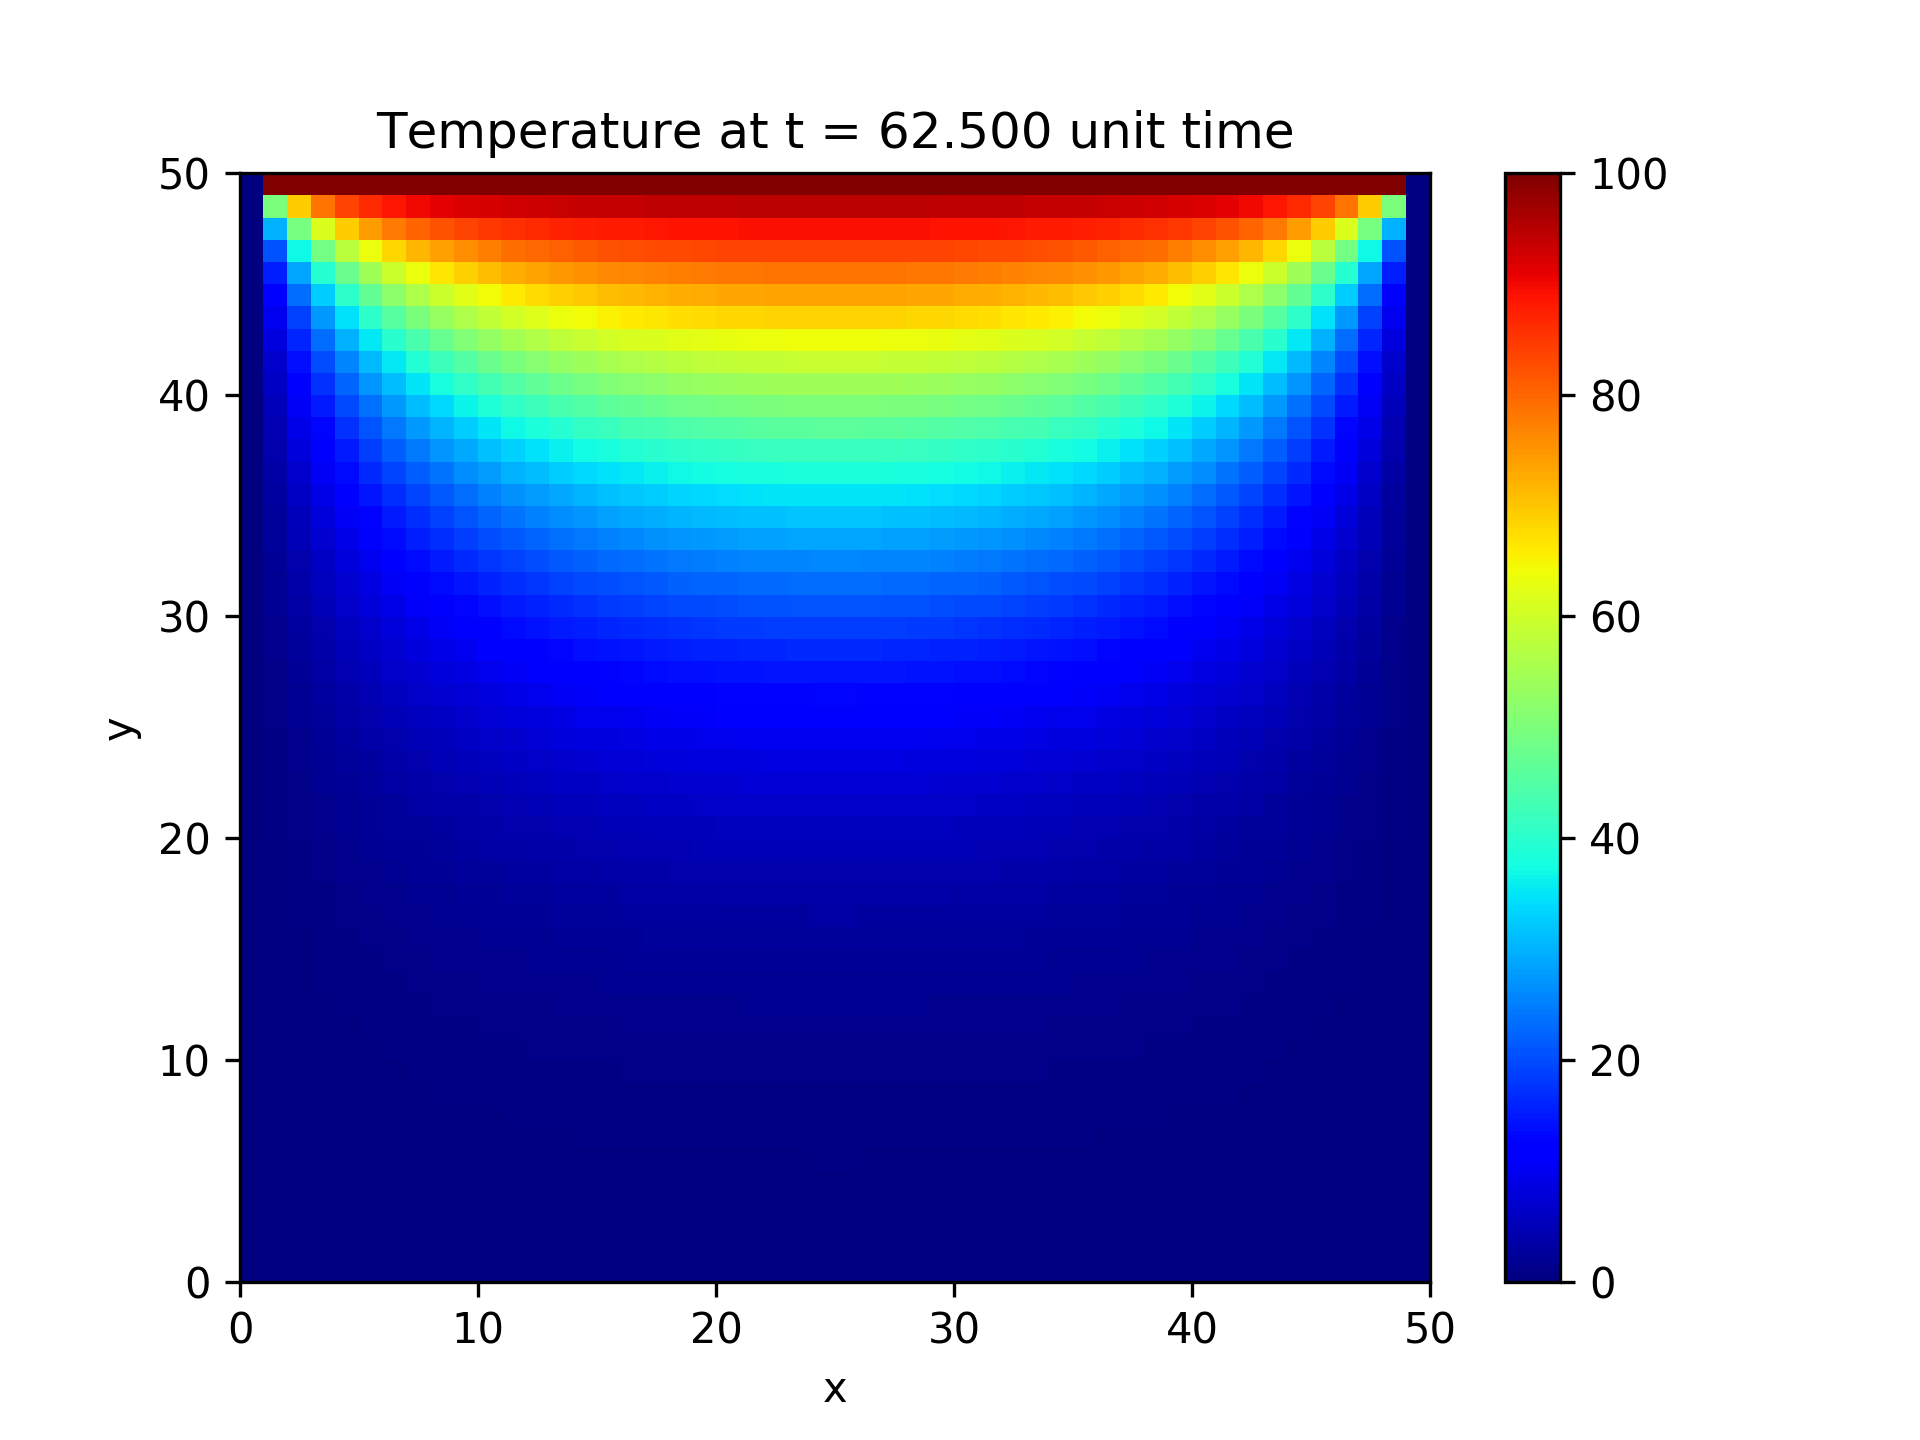
\includegraphics[width=0.7\textwidth]{figures/frame500}
	\caption{Situation after about 60 seconds.}
	\label{fig:heat_end_1}
\end{figure} 

As a second example, let’s set all of the boundary conditions to 0, and then randomize the initial condition for the interior grid (below only the updated part of the code is shown for brevity).

\begin{ipython}
...
# Initial condition everywhere inside the grid
#u_initial = 0
u_initial = np.random.uniform(low=28.5, high=55.5, size=(plate_length,plate_length))

# Change initial conditions
#u.fill(u_initial)
u[0,:,:] = u_initial

# Boundary conditions
u_top = 0.0
u_left = 0.0
u_bottom = 0.0
u_right = 0.0

# Set the initial condition
u.fill(u_initial)
...
\end{ipython}

In this second case, being the interior initially warmer it cools down as time goes by. Figure~\ref{fig:heat_2} shows the initial condition and the situation after about 30 seconds.
 
\begin{figure}[htb]
	\centering
	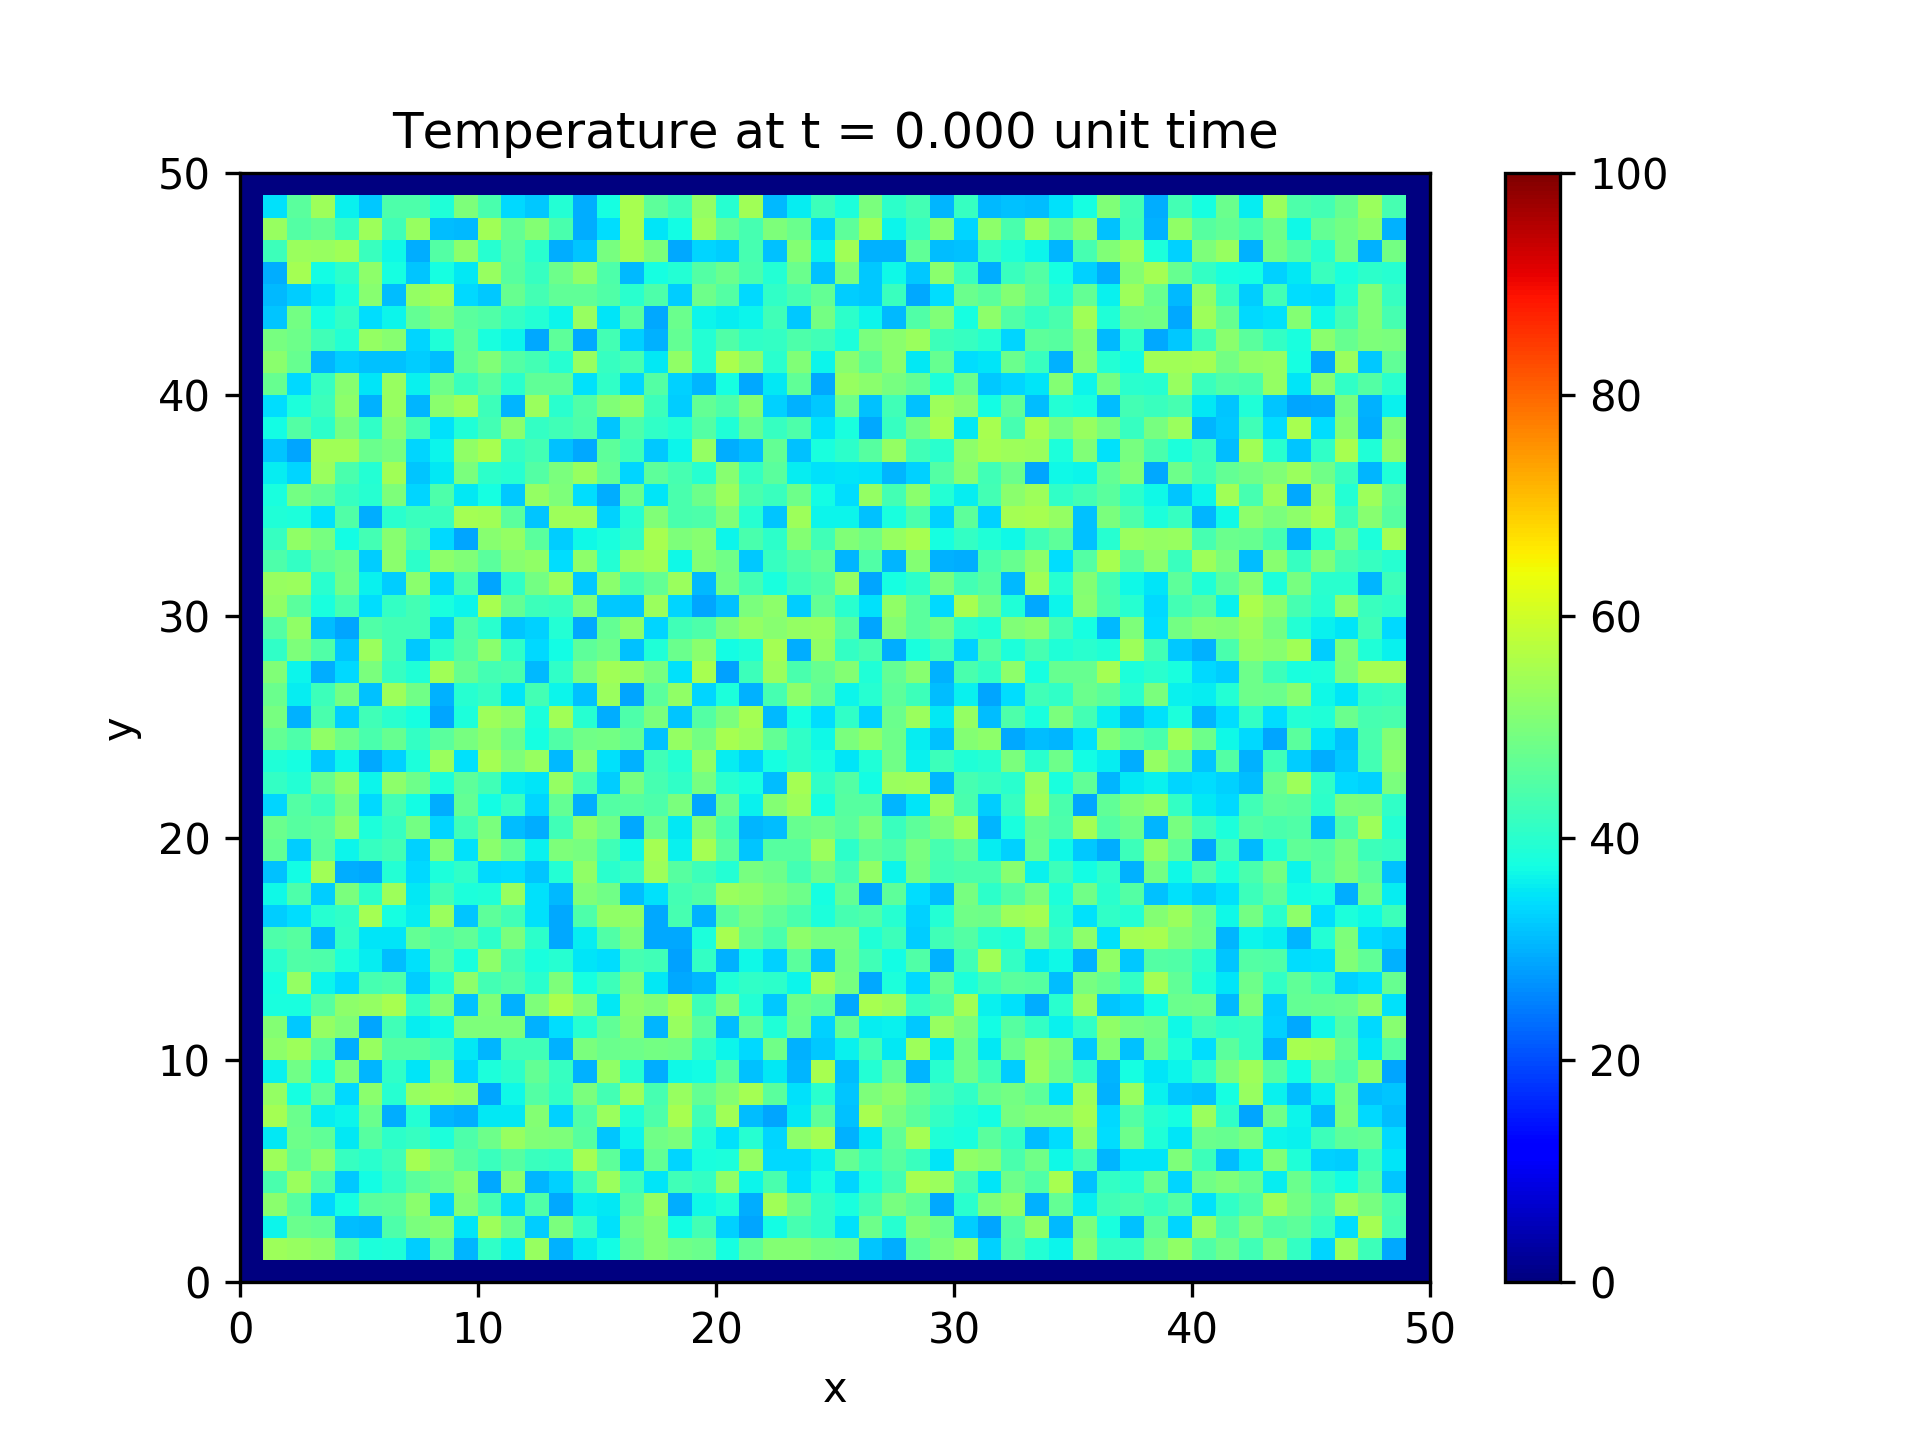
\includegraphics[width=0.45\textwidth]{figures/frame0_2}
	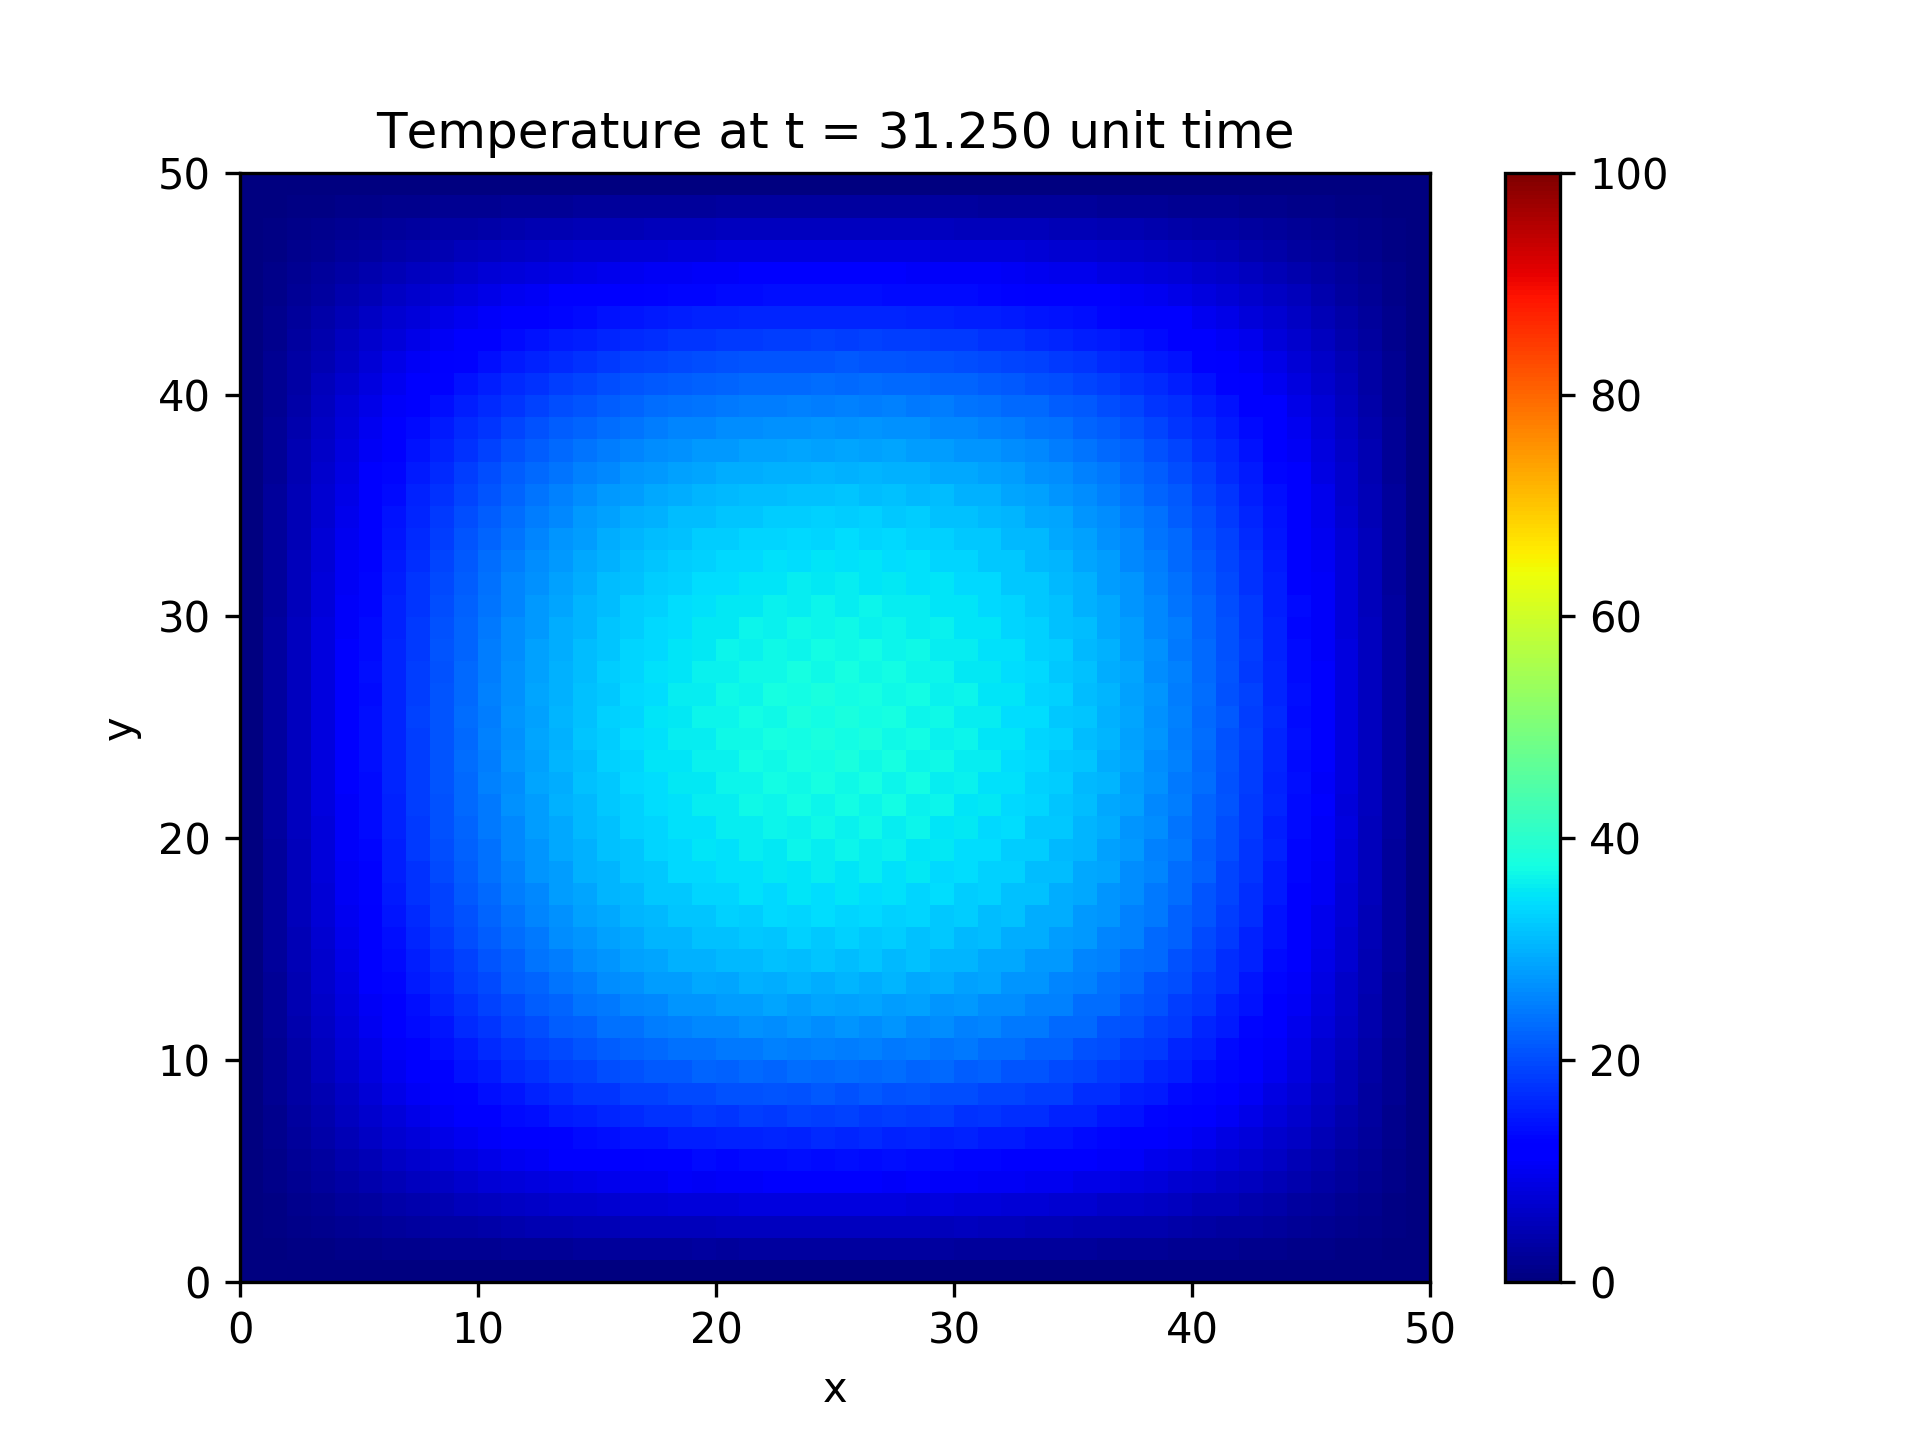
\includegraphics[width=0.45\textwidth]{figures/frame250_2}
	\caption{Initial condition of the second example of heat equation solution (left), heat distribution after after about 31.25 seconds (right).}
	\label{fig:heat_2}
\end{figure} 

\subsection{Alternative Formulation}
In the heat equation (one-dimensional) replace
\begin{equation}
\cfrac{\partial y_{i,j}}{\partial t} = \cfrac{\partial y_{x_i, t_j}}{\partial t} = \cfrac{y_{i,j+1} − y_{i,j}}{\Delta t}
\end{equation}
\noindent 
and
\begin{equation}
\cfrac{\partial^2 y_{i,j}}{\partial x^2}=\cfrac{y_{i+1,j} − 2y_{i,j} + y_{i−1,j}}{\Delta x^2}
\end{equation}
\noindent
which leads to the \emph{difference equation}
\begin{equation}
\cfrac{y_{i,j+1} - y_{i,j}}{\Delta t} = \cfrac{y_{i+1,j} − 2y_{i,j} + y_{i−1,j}}{\Delta x^2}
\end{equation}
\noindent
In case all values $y$ are calculated for the time level $j$, then the values of the time level $j + 1$ are given by
\begin{equation}
y_{i,j+1} = y_{i,j} + \cfrac{\Delta t}{\Delta x^2} \left(y_{i+1,j} − 2y_{i,j} + y_{i−1,j}\right)
\end{equation}

With the notation $\alpha = \Delta t/\Delta x^2$
\begin{equation}
y_{i,j+1} = \alpha y_{i−1,j} + (1 − 2\alpha)y_{i,j} + \alpha y_{i+1,j} 
\label{eq:explicit_formula}
\end{equation}
Eq.~\ref{eq:explicit_formula} can be generalized as
\begin{equation}
y_{i,j+1} = a_i y_{i−1,j} + b_i y_{i,j} + c_i y_{i+1,j} 
\label{eq:explicit_formula}
\end{equation}
\noindent
which suggests the possibility that it may be written also in matrix notation
\begin{equation}
Y_{i+1} + K_i = [A]Y_i \quad i=N-1, 2,\ldots,2,0
\end{equation}
\noindent
where
\begin{equation*}
Y_i =
\begin{bmatrix}
y_{i, 1}\\
y_{i, 2}\\
\vdots\\
\vdots\\
y_{i,N-1}\\
\end{bmatrix},
K_i=
\begin{bmatrix}
-a_1 y_{i,0}\\
0\\
\vdots\\
0\\
-c_{M-1}y_{i,N}
\end{bmatrix},
[A] = 
\begin{bmatrix}
b_1 & c_1 & 0 \cdots & 0 & 0 & 0 \\
a_2 & b_2 & c_2 \cdots & 0 & 0 & 0\\
0  & a_3 & b_3 & c_3\cdots & 0 & 0 \\
0  & \vdots & \vdots & \ddots & \vdots & 0 \\
0 & 0 & 0 & \cdots & a_{M-1} & b_{M-1} \\
\end{bmatrix}
\end{equation*}

This is equivalent to a system of equations that can be solved using the method explained in Chapter~\ref{matrix-equations}.

\subsubsection{Example of Instability}
Consider again the heat equation (1D this time)

\begin{equation}
\cfrac{\partial y}{\partial t} = \cfrac{\partial^2 y}{\partial x^2}
\end{equation}
\noindent
with $y(x, 0) = \textrm{sin}\pi x$, $x_{0} = 0$, $x_M = 1$ and boundary conditions $= 0$. Let us approximate $y(x = 0.2, t = 0.5)$ using a grid with $\Delta x = 0.1$ (i.e. $M = 10$ and $0.2 = x_2$, and two different values of $\Delta t$: 0.0005 and 0.01.

\begin{ipython}
import numpy as np
import math

def example(V, N, M, alpha):
    for j in np.arange(N):
        for i in range(1, M):
            V[j+1, i] = alpha*V[j, i-1] + (1-2*alpha)*V[j, i] + alpha*V[j, i+1]
    return V

N = 1000 #50 
M = 10
dt = 0.5/N
dx = 1/M
alpha = dt/dx**2
x = np.linspace(0, 1, M+1)
y = np.zeros(shape=(N+1, M+1))
y[0,:] = np.sin(math.pi*x)

y_exp = example(y, N, M, alpha)
print (y[int(0.5/dt), int(0.2/dx)])
\end{ipython}
\noindent
Running with $N=50$ gives
\begin{ioutput}
0.004349220987439513
\end{ioutput}
\noindent
Running with $N=50$ gives
\begin{ioutput}
-466863.4978153779
\end{ioutput}

\begin{itemize}
\item $\Delta t = 0.0005 \implies \alpha = 0.05$ yields $y_{2,1000}=0.00435$;
\item $\Delta t = 0.01 \implies \alpha = 1$ yields $y_{2,50}=-5\cdot 10^5$
\end{itemize}
Hence there is an instability, i.e. different results according to grid granularity.

If $y(j)$ denotes the exact solution of $y(j+1) = [A] y(j) + d(j)$, $\bar{y}(j)$ the approximated solution (i.e. including all errors), $e(j) = y(j)-\bar{y}(j)$ and
\begin{equation}
r(j+1) = \bar{y}(j+1) − [A]y(j) − d(j)
\end{equation}
\noindent
the vector $r(j+1)$ represents the error at the j$^{th}$ step. %, and it suffices to study the propagation of one such errors to understand the behavior of the method. So we set $r(j) = 0$ for $j > 1$, i.e. study propagation of the error $e(0)$ in the course of the iterations.

\begin{equation}
\begin{split}
y(j+1) &= [A]y(j) + d(j),\quad (j > 1) \\
&\implies [A]e(j) = [A]\bar{y}(j) − [A]y(j) = \bar{y}(j+1) − y(j+1) = e(j+1) \\
&\implies e(j) = [A]^j e(0)
\end{split}
\end{equation}
For stable behavior, is required that $[A]^j e(0) \rightarrow 0$ for $j\rightarrow\infty$.

It is possible to demonstrate that for $0\lt \alpha\leq\cfrac{1}{2}$ the explicit method $y(j+1) = [A]y(j)$ is stable.
Since $\alpha=\cfrac{\Delta t}{\Delta x^2}$ this result implies that the step sizes $\Delta t$ and $\Delta x$  cannot be chosen independent of each other.
Indeed if accuracy is improved by halving the $\Delta x$ price step, time step must be reduced by a factor of four or more (and the computation time goes up by a factor of eight). The improvement in accuracy we would get from such a reduction in step sizes is a factor of four since the explicit finite-difference method is accurate to $O(\Delta t) + O(\Delta x^2)$.

Concerning stability, it can be proved that the implicit method is \emph{unconditionally} stable and that $\Delta t$ and $\Delta x$ can be chosen independent of each other.
On the other hand a weakness of this method is the accuracy of the first order in $\Delta t$ (the error is of the order of $O(\Delta x^2) + O(\Delta t)$). 

Finally the Crank-Nicolson method is proved to be stable with an error $O(\Delta t^2)$. 

In conclusion the advantages of the explicit method can be summarized as follows:
\begin{itemize}
\tightlist
\item it is very easy to program and hard to make mistakes;
\item it copes well with coefficients that are asset and/or time-dependent;
\item American options are easily implemented (see next Section);
\item it is relatively fast.
\end{itemize}

Its main disadvantage is the restriction on time step choice because of the stability issues seen above which can affect the speed of the algorithm.

Implicit finite difference methods are usually used to overcome the stability issue. There is no more need for ridiculously small time-steps. But the solution is not so straightforward. With a little extra computational effort the implicit method precision can be improved significantly (at least in theory) by using Crank-Nicolson method. 

\section{European Options}
Let's introduce again the Black-Scholes (BS) equation, see also Chapter~\ref{ch:BS}

\begin{equation}
\cfrac{\partial V}{\partial t} + \cfrac{1}{2} \sigma^2 S^2 \cfrac{\partial^2 V}{\partial S^2}+ rS \cfrac{\partial V}{\partial S} − rV = 0
\label{eq:bs_differential_equation}
\end{equation}
\noindent
where $V$ stands for the price of the option, $S$ denotes the current value of the underlying assets, $\sigma$ its volatility, $t$ is time and $r$ the risk-free interest rate.

The BS equation is aimed at calculating the price of an option, and the only unknown here is the price of this option ($V$), depending on $S$ and $t$. In the next Sections we will use finite difference method to solve this nonlinear second-order parabolic equation.

\subsection{Boundary Conditions}
Consider an European call option $C(S, t)$ of a stock at the expiry time $t=T$. Its payoff is given by $C(S, T) = \textrm{max}(S-K, 0)$. This is the final condition for the Black-Scholes equation, however, usually it is preferred to deal with an initial condition with a form  $C(S,0)=f(S)$. So we can apply a change of variable

\begin{equation}
t^* = T - t \rightarrow \cfrac{\partial V}{\partial t} = -\cfrac{\partial V}{\partial t^*} 
\end{equation}
\noindent
which substituted in the BS equation gives
\begin{equation}
\cfrac{\partial V}{\partial t^*} - \cfrac{1}{2} \sigma^2 S^2 \cfrac{\partial^2 V}{\partial S^2} - rS \cfrac{\partial V}{\partial S} + rV = 0
\end{equation}
\noindent
with initial condition $V(S,0)=\textrm{max}(S-K, 0)$. Be careful that this initial condition reflects the expiry moment $t=T$ and when we are stepping forward to calculate the last time step in $t^*$ we are actually calculating the price of the call option at $t=0$ (i.e. time transformation $t\rightarrow t^*$ converts the terminal condition for $V(S, T) = V(S, t^*)$ to an initial condition for $t^* = 0$).

In order to make it a well-posed partial differential equation, we need to define the boundary conditions on both sides in the variable $S$. The current price of the stock can take values in the interval $[0, \infty)$ which is unbounded. However, in the numerical method, we need to set an artificial bound $S_{max}$ otherwise we will have an infinite number of grid points. Usually it is recommended to set $S_{max}$ around four times the exercise price $K$ ($S_{max} = 4K$).

So in conclusion the boundary conditions can be written as
\begin{equation}
\begin{cases}
V(0, t^*) = 0 \\
V(S_{max}, t^*) = S_{max} - K \\
\end{cases}
\end{equation}

The discretized version of each term of the BS equation are
\begin{gather}
\cfrac{\partial V}{\partial t^*} = \cfrac{V_{i, n+1}-V_{i, n}}{\Delta t} \\
\cfrac{\partial V}{\partial S} = \cfrac{V_{i+1, n}-V_{i-1, n}}{2\Delta S} \\
\cfrac{\partial^2 V}{\partial S^2} = \cfrac{V_{i+1, n}-2V_{i, n}+V_{i-1, n}}{\Delta S^2}
\end{gather}
\noindent
which substituted into Eq.~\ref{eq:bs_differential_equation} give
\begin{equation}
\cfrac{V_{i, n+1}-V_{i, n}}{\Delta t} - \cfrac{1}{2}\sigma^2 S^2
\cfrac{V_{i+1, n}-2V_{i, n}+V_{i-1, n}}{\Delta S^2} - rS
\cfrac{V_{i+1,n}-V_{i-1,n}}{2\Delta S} + rV_{i,n} = 0
\end{equation}

Since $S=i\Delta S$ we can rearrange the above equation as:
\begin{equation}
\cfrac{V_{i, n+1}-V_{i, n}}{\Delta t} - \cfrac{1}{2}\sigma^2 i^2
\left(V_{i+1, n}-2V_{i, n}+V_{i-1, n}\right) - \cfrac{1}{2}ri
\left(V_{i+1,n}-V_{i-1,n}\right) + rV_{i,n} = 0
\end{equation}
\noindent
and the option price at the next time step can be expressed as
\begin{equation}
V_{i, n+1} = \cfrac{1}{2}\left(\sigma^2 i^2+ri\right)V_{i+1,n} \Delta t +
\left(1-\sigma^2 i^2\Delta t-r\Delta t \right)V_{i,n} +
\cfrac{1}{2}\left(\sigma^2 i^2 - ri\right)V_{i-1,n} \Delta t
\end{equation}

This difference equation can be easily implemented in \texttt{python}.
\begin{ipython}
import numpy as np

class FiniteDifference:
    def __init__(self, M, N, Smin, Smax, T, K, r, D, sigma):
        self.r = r
        self.K = K
        self.D = D
        self.sigma = sigma
        self.M = M
        self.N = N
        self.V = np.zeros(shape=(M+1,N+1))   
        self.dt = T/N
        self.dS = (Smax - Smin)/M

        self.S = np.linspace(Smin, Smax, M+1)
        self.t = np.linspace(0, T, N+1)

        self.V[:, 0] = np.maximum(self.S-self.K, 0)
        self.V[0, :] = 0
        self.V[self.M, :] = self.Smax*np.exp(-self.D*self.t) - \
                            self.K*np.exp(-self.r*self.t)

    def explicit(self):
        for j in range(self.N):
            for i in range(1, self.M):
                self.V[i, j+1] = 0.5*self.dt*(self.sigma*self.sigma*i*i-\
                                 (self.r-self.D)*i)*self.V[i-1, j]+(1-self.dt* \
                                 (self.sigma*self.sigma*i*i+self.r))*self.V[i, j]+\
                                 0.5*self.dt*(self.sigma*self.sigma*i*i+\
                                 (self.r-self.D)*i)*self.V[i+1, j]
\end{ipython}             

As an example consider a European call with an underlying currently traded at \$20 (with a volatility of 0.2). The maturity is six months, the strike price is \$10 and the risk-free interest rate is 10\%. Let's compute the price of the option.
\begin{ipython}
fd = FiniteDifference(100, 300, 0, 30, 1, 10, 0.2, 0, 0.1)
fd.explicit()
\end{ipython}

Figure~\ref{fig:bs_finite_difference} shows the call option price against the current stock price. As a comparison the same plot obtained with the analytical solution of the Black-Scholes equation is also shown. 

\begin{figure}[htb]
	\centering
	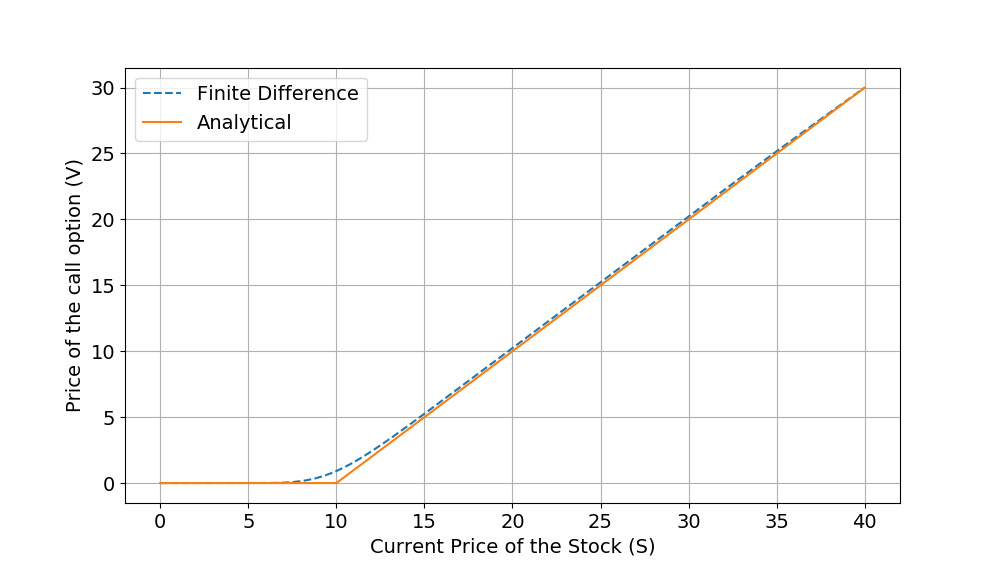
\includegraphics[width=0.7\textwidth]{figures/bs_finite_difference}
	\caption{Comparison between the analytical solution and the option price obtained with the explicit finite difference method.}
	\label{fig:bs_finite_difference}
\end{figure} 

Figure~\ref{fig:explicit_relative_error} reports the error on the option price computed with the explicit finite difference method relative to the analytical calculation obtained from the Black-Scholes model. The most obvious conclusion that can be made from the plot is that the error is larger when the option is at-the-money. Also error depends on $\sigma$ and $r$. Of course the relationship between $dS$ and $dt$ have crucial influence to the stability of the' explicit method. 
 
\begin{figure}[htb]
	\centering
	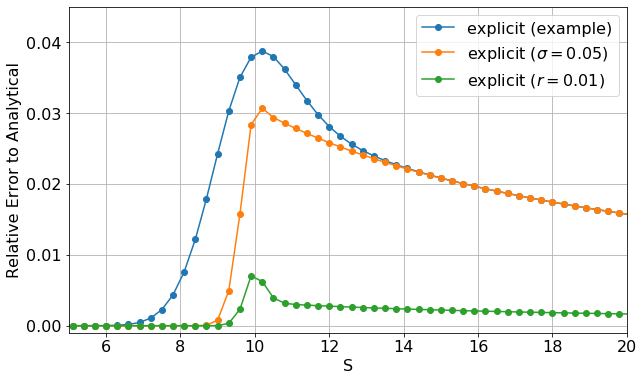
\includegraphics[width=0.7\textwidth]{figures/explicit_relative_error}
	\caption{Relative error between option price computed with explicit finite difference method and analytically using Black-Scholes formula.}
	\label{fig:explicit_relative_error}
\end{figure} 

\section{American Options}
The main characteristic of an American option is the possibility of early exercise. 
The explicit finite difference method can be easily adapted to account for this additional feature not available in European options.

After each iteration it is indeed enough to compare the calculated option value with the it intrinsic value, taking the larger of the two. The \texttt{python} class can be adapted accordingly (a parameter to set call or put has been added too):
\begin{ipython}
import numpy as np

class FiniteDifference:
    def __init__(self, M, N, Smin, Smax, T, K, r, D, sigma, 
                 iscall=True, isamerican=False):
        self.iscall = iscall
        self.isamerican = isamerican
        self.r = r
        self.K = K
        self.D = D
        self.sigma = sigma
        self.M = M
        self.N = N
        self.V = np.zeros(shape=(M+1,N+1))   
        self.dt = T/N
        self.dS = (Smax - Smin)/M

        self.S = np.linspace(Smin, Smax, M+1)
        self.t = np.linspace(0, T, N+1)

        if self.iscall:
            self.V[:, 0] = np.maximum(self.S - self.K, 0)
            self.V[self.M, :] = Smax*np.exp(-self.D*self.t) - \
                                self.K*np.exp(-self.r*self.t)
            self.V[0, :] = 0
        else:
            self.V[:, 0] = np.maximum(self.K - self.S, 0)
            self.V[self.M, :] = self.K*np.exp(-self.r*self.t) - \
                                Smax*np.exp(-self.D*self.t)

    def explicit(self):
        for j in range(self.N):
            for i in range(1, self.M):
                self.V[i, j+1] = 0.5*self.dt*(self.sigma*self.sigma*i*i-\
                                 (self.r-self.D)*i)*self.V[i-1, j]+(1-self.dt* \
                                 (self.sigma*self.sigma*i*i+self.r))*self.V[i, j]+\
                                 0.5*self.dt*(self.sigma*self.sigma*i*i+\
                                 (self.r-self.D)*i)*self.V[i+1, j]
            if self.isamerican:
                V[:, j+1] = np.maximum(V[:, j+1], V[:, 0])
\end{ipython}             

Consider now an American call with an underlying currently traded at \$20 (with a volatility of 0.2). The maturity is six months, the strike price is \$10 and the risk-free interest rate is 10\% and the dividend rate is 5\%. Let's compute the price of the option.
\begin{ipython}
fd = FiniteDifference(100, 300, 0, 30, 1, 10, 0.2, 0.05, 0.1, True, True)
fd.explicit()
\end{ipython}

Figure~\ref{fig:american_call_surface} shows the American option price surface for the call used in the example above.
\begin{figure}[htb]
	\centering
	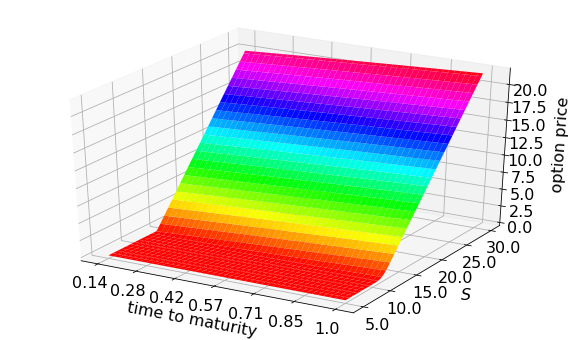
\includegraphics[width=0.7\textwidth]{figures/american_call_surface}
	\caption{Option price surface.}
	\label{fig:american_call_surface}
\end{figure} 

\section{Exercises}
\input{numerical_approx_ex_text}

\begin{thebibliography}{9}
\bibitem{bib:ode}\href{https://en.wikipedia.org/wiki/Ordinary_differential_equation}{\emph{Ordinary differential equation}}, Wikipedia [Online]
\end{thebibliography}


% \section{Finite Differences in Option Pricing}
%The motivation behind the finite differencing is the application of the Black-Scholes Partial Differential Equation (PDE) framework (involving functions and their partial derivatives) whose price $S(t)$ is a function of
%$f(S,t)$, with $r$ as the risk-free rate, $t$ as the time to maturity, and $\sigma$ as the volatility of the underlying security:
%
%\begin{equation}
%rf = \cfrac{\partial f}{\partial t} + rS\cfrac{\partial f}{\partial S} + \cfrac{1}{2} \sigma^2 S^2 \cfrac{\partial ^2 f}{\partial t^2}
%\end{equation}
%
%The finite difference technique tends to converge faster than lattices and approximates complex exotic options very well.
%To solve a PDE by finite differences working backward in time, a discrete-time grid of size $M$ by $N$ is set up to reflect asset prices over a course of time, such that $S$ and
%$t$ take on the following values at each point on the grid:
%
%\begin{equation}
%\begin{gathered}
%S = 0, dS, 2dS, 3dS,\ldots, (M −1) dS, S_{max} \\
%t = 0, dt, 2dt, 3dt,\ldots (N −1) dt, T
%\end{gathered}
%\end{equation}
%
%It follows that by grid notation, $f_{i, j} = f (idS, jdt)$. $S_{max}$ is a suitably large asset price that cannot be reached by the maturity time, $T$. $dS$ and $dt$ are thus intervals between each node in the grid, incremented by price and time respectively. The terminal condition at expiration time $T$ for every value of $S$ is $\textrm{max}(S − K,0)$ for a call option with strike $K$ and $\textrm{max}(K − S,0)$ for a put option. The grid traverses backward from the terminal conditions, complying with the PDE while adhering to the boundary conditions of the grid, such as the payoff from an early exercise.
%
%The boundary conditions are defined values at the extreme ends of the nodes, where $i=0$ and $i=N$ for every time at $t$. Values at the boundaries are used to calculate the values of all other lattice nodes iteratively using the PDE.
%
%A visual representation of the grid is given by the following figure. As $i$ and $j$ increase from the top-left corner of the grid, the price $S$ tends toward $S_{max}$ (the maximum price possible) at the bottom-right corner of the grid:
%A number of ways to approximate the PDE are as follows: 
%
%\begin{itemize}
%\item Forward difference:
%\begin{equation}
%\cfrac{\partial f}{\partial S} = \cfrac{f_{i+1,j} − f_{i,j}}{\partial S},\quad \cfrac{\partial f}{\partial t} = \cfrac{f_{i,j+1} − f_{i,j}}{\partial t}
%\end{equation}
%
%\item Backward difference:
%\begin{equation}
%	\cfrac{\partial f}{\partial S} = \cfrac{f_{i,j} − f_{i-1,j}}{\partial S},\quad \cfrac{\partial f}{\partial t} = \cfrac{f_{i,j} − f_{i,j-1}}{\partial t}
%\end{equation}
%
%\item Central or symmetric difference:
%\begin{equation}
%	\cfrac{\partial f}{\partial S} = \cfrac{f_{i+1,j} − f_{i-1,j}}{2\partial S},\quad \cfrac{\partial f}{\partial t} = \cfrac{f_{i,j+1} − f_{i,j-1}}{2\partial t}
%\end{equation}
%
%\item The second derivative:
%\begin{equation}
%	\cfrac{\partial^2 f}{\partial S^2} = \cfrac{f_{i+1,j} − 2f_{i,j} +  f_{i-1,j}}{2\partial S^2}
%\end{equation}
%\end{itemize}
%
%Once we have the boundary conditions set up, we can now apply an iterative approach using the explicit, implicit, or Crank-Nicolson method.
%
%\subsection{The Explicit Method}
%The explicit method for approximating $f_{i, j}$ is given by:
%
%\begin{equation}
%rf_{i,j} = \cfrac{f_{i,j} − f_{i,j−1}}{dt} + ridS \cfrac{f_{i+1,j} − f_{i−1,j}}{2dS} +\cfrac{1}{2} \sigma^2 j^2 \cfrac{f_{i+1,j} + f_{i−1,j}}{dS^2}
%\end{equation}
%
%Here, it can be seen that the first difference is the backward difference with respect to $t$, the second difference is the central difference with respect to $S$, and the third difference is the second-order difference with respect to $S$. When we rearrange the terms, we have the following equation:
%
%\begin{equation}
%f_{i,j} =a^* f_{i-1,j+1} +b^* f_{i,j+1} +c^* f_{i+1,j+1}
%\end{equation}
%where $j=N−1,N−2,N−3,\ldots, 2,1,0$ and $i=1,2,3,\ldots, M−2,M−1$:
%
%\begin{equation}
%\begin{gathered}
%a^* = \cfrac{1}{2}dt(\sigma^2 i^2 −ri)\\
%b^* =1−dt(\sigma^2 i^2 −ri) \\
%c^* = \cfrac{1}{2}dt(\sigma^2 i^2 +ri)
%\end{gathered}	
%\end{equation} 
% 
%The iterative approach of the explicit method can be visually represented by the following figure:
%
%\begin{center}
%\begin{tikzpicture}
%	[parent anchor=east,child anchor=west,grow=east]
%	%\tikzstyle{every node}=[ball color=red,circle,text=white]
%	\tikzstyle{edge from parent}=[draw,ultra thick,red]
%	\node {$f_{i,j}$}
%	child {node {$f_{i+1,j+1}$}}
%	child {node {$f_{i,j+1}$}}
%	child {node {$f_{i-1,j+1}$}};
%\end{tikzpicture}
%\end{center}
%
%\subsection{\texttt{FiniteDifferences} class}
%As we will be writing the explicit, implicit, and Crank-Nicolson methods of finite differences in \texttt{python}, let's write a parent class that can inherit the common properties and functions of all three methods.
%
%We will create a class called \texttt{FiniteDifferences} that accepts and assigns all the required parameters in the constructor method.
%
%\begin{codebox}
%\begin{Verbatim}[commandchars=\\\{\}]
%\PY{k+kn}{import} \PY{n+nn}{numpy} \PY{k}{as} \PY{n+nn}{np}
%		
%\PY{k}{class} \PY{n+nc}{FiniteDifferences}\PY{p}{:}
%    \PY{k}{def} \PY{n+nf+fm}{\PYZus{}\PYZus{}init\PYZus{}\PYZus{}}\PY{p}{(}\PY{n+nb+bp}{self}\PY{p}{,} \PY{n}{S0}\PY{p}{,} \PY{n}{K}\PY{p}{,} \PY{n}{r}\PY{p}{,} \PY{n}{T}\PY{p}{,} \PY{n}{sigma}\PY{p}{,} \PY{n}{Smax}\PY{p}{,} \PY{n}{M}\PY{p}{,} \PY{n}{N}\PY{p}{,} \PY{n}{is\PYZus{}call} \PY{o}{=} \PY{k+kc}{True}\PY{p}{)}\PY{p}{:}
%        \PY{n+nb+bp}{self}\PY{o}{.}\PY{n}{S0} \PY{o}{=} \PY{n}{S0}
%        \PY{n+nb+bp}{self}\PY{o}{.}\PY{n}{K} \PY{o}{=} \PY{n}{K}
%        \PY{n+nb+bp}{self}\PY{o}{.}\PY{n}{r} \PY{o}{=} \PY{n}{r}
%        \PY{n+nb+bp}{self}\PY{o}{.}\PY{n}{T} \PY{o}{=} \PY{n}{T}
%        \PY{n+nb+bp}{self}\PY{o}{.}\PY{n}{sigma} \PY{o}{=} \PY{n}{sigma}
%        \PY{n+nb+bp}{self}\PY{o}{.}\PY{n}{Smax} \PY{o}{=} \PY{n}{Smax}
%        \PY{n+nb+bp}{self}\PY{o}{.}\PY{n}{M}\PY{p}{,} \PY{n+nb+bp}{self}\PY{o}{.}\PY{n}{N} \PY{o}{=} \PY{n+nb}{int}\PY{p}{(}\PY{n}{M}\PY{p}{)}\PY{p}{,} \PY{n+nb}{int}\PY{p}{(}\PY{n}{N}\PY{p}{)}
%        \PY{n+nb+bp}{self}\PY{o}{.}\PY{n}{is\PYZus{}call} \PY{o}{=} \PY{n}{is\PYZus{}call}
%        \PY{n+nb+bp}{self}\PY{o}{.}\PY{n}{dS} \PY{o}{=} \PY{n}{Smax} \PY{o}{/} \PY{n+nb}{float}\PY{p}{(}\PY{n+nb+bp}{self}\PY{o}{.}\PY{n}{M}\PY{p}{)}
%        \PY{n+nb+bp}{self}\PY{o}{.}\PY{n}{dt} \PY{o}{=} \PY{n}{T} \PY{o}{/} \PY{n+nb}{float}\PY{p}{(}\PY{n+nb+bp}{self}\PY{o}{.}\PY{n}{N}\PY{p}{)}
%        \PY{n+nb+bp}{self}\PY{o}{.}\PY{n}{i\PYZus{}values} \PY{o}{=} \PY{n}{np}\PY{o}{.}\PY{n}{arange}\PY{p}{(}\PY{n+nb+bp}{self}\PY{o}{.}\PY{n}{M}\PY{p}{)}
%        \PY{n+nb+bp}{self}\PY{o}{.}\PY{n}{j\PYZus{}values} \PY{o}{=} \PY{n}{np}\PY{o}{.}\PY{n}{arange}\PY{p}{(}\PY{n+nb+bp}{self}\PY{o}{.}\PY{n}{N}\PY{p}{)}
%        \PY{n+nb+bp}{self}\PY{o}{.}\PY{n}{grid} \PY{o}{=} \PY{n}{np}\PY{o}{.}\PY{n}{zeros}\PY{p}{(}\PY{n}{shape}\PY{o}{=}\PY{p}{(}\PY{n+nb+bp}{self}\PY{o}{.}\PY{n}{M}\PY{o}{+}\PY{l+m+mi}{1}\PY{p}{,} \PY{n+nb+bp}{self}\PY{o}{.}\PY{n}{N}\PY{o}{+}\PY{l+m+mi}{1}\PY{p}{)}\PY{p}{)} 
%        \PY{n+nb+bp}{self}\PY{o}{.}\PY{n}{boundary\PYZus{}conds} \PY{o}{=} \PY{n}{np}\PY{o}{.}\PY{n}{linspace}\PY{p}{(}\PY{l+m+mi}{0}\PY{p}{,} \PY{n}{Smax}\PY{p}{,} \PY{n+nb+bp}{self}\PY{o}{.}\PY{n}{M}\PY{o}{+}\PY{l+m+mi}{1}\PY{p}{)}
%		
%    \PY{k}{def} \PY{n+nf}{\PYZus{}setup\PYZus{}boundary\PYZus{}conditions\PYZus{}}\PY{p}{(}\PY{n+nb+bp}{self}\PY{p}{)}\PY{p}{:}
%        \PY{k}{pass}
%		
%    \PY{k}{def} \PY{n+nf}{\PYZus{}setup\PYZus{}coefficients\PYZus{}}\PY{p}{(}\PY{n+nb+bp}{self}\PY{p}{)}\PY{p}{:}
%        \PY{k}{pass}
%		
%    \PY{k}{def} \PY{n+nf}{\PYZus{}traverse\PYZus{}grid\PYZus{}}\PY{p}{(}\PY{n+nb+bp}{self}\PY{p}{)}\PY{p}{:}
%        \PY{k}{pass}
%		
%    \PY{k}{def} \PY{n+nf}{\PYZus{}interpolate\PYZus{}}\PY{p}{(}\PY{n+nb+bp}{self}\PY{p}{)}\PY{p}{:}
%        \PY{k}{return} \PY{n}{np}\PY{o}{.}\PY{n}{interp}\PY{p}{(}\PY{n+nb+bp}{self}\PY{o}{.}\PY{n}{S0}\PY{p}{,} \PY{n+nb+bp}{self}\PY{o}{.}\PY{n}{boundary\PYZus{}conds}\PY{p}{,} \PY{n+nb+bp}{self}\PY{o}{.}\PY{n}{grid}\PY{p}{[}\PY{p}{:}\PY{p}{,} \PY{l+m+mi}{0}\PY{p}{]}\PY{p}{)}
%		
%    \PY{k}{def} \PY{n+nf}{price}\PY{p}{(}\PY{n+nb+bp}{self}\PY{p}{)}\PY{p}{:} 
%        \PY{n+nb+bp}{self}\PY{o}{.}\PY{n}{\PYZus{}setup\PYZus{}boundary\PYZus{}conditions\PYZus{}}\PY{p}{(}\PY{p}{)} 
%        \PY{n+nb+bp}{self}\PY{o}{.}\PY{n}{\PYZus{}setup\PYZus{}coefficients\PYZus{}}\PY{p}{(}\PY{p}{)} 
%        \PY{n+nb+bp}{self}\PY{o}{.}\PY{n}{\PYZus{}traverse\PYZus{}grid\PYZus{}}\PY{p}{(}\PY{p}{)}
%        \PY{k}{return} \PY{n+nb+bp}{self}\PY{o}{.}\PY{n}{\PYZus{}interpolate\PYZus{}}\PY{p}{(}\PY{p}{)}
%\end{Verbatim}
%\end{codebox}
%
%All of these methods are protected methods and may be overwritten by derived classes. The pass keyword simply does nothing; the derived classes will provide specific implementations of these functions.
%
%\subsubsection{\texttt{FDExplicitEu} class}
%
%The \texttt{python} implementation of finite differences by the explicit method is given in the following \texttt{FDExplicitEu} class, which inherits from the \texttt{FiniteDifferences} class and overrides the required implementation methods.
%
%\begin{codebox}
%\begin{Verbatim}[commandchars=\\\{\}]
%\PY{k+kn}{import} \PY{n+nn}{numpy} \PY{k}{as} \PY{n+nn}{np}
%		
%\PY{k}{class} \PY{n+nc}{FDExplicitEu}\PY{p}{(}\PY{n}{FiniteDifferences}\PY{p}{)}\PY{p}{:}
%    \PY{k}{def} \PY{n+nf}{\PYZus{}setup\PYZus{}boundary\PYZus{}conditions\PYZus{}}\PY{p}{(}\PY{n+nb+bp}{self}\PY{p}{)}\PY{p}{:} 
%        \PY{k}{if} \PY{n+nb+bp}{self}\PY{o}{.}\PY{n}{is\PYZus{}call}\PY{p}{:}
%            \PY{n+nb+bp}{self}\PY{o}{.}\PY{n}{grid}\PY{p}{[}\PY{p}{:}\PY{p}{,} \PY{o}{\PYZhy{}}\PY{l+m+mi}{1}\PY{p}{]} \PY{o}{=} \PY{n}{np}\PY{o}{.}\PY{n}{maximum}\PY{p}{(}\PY{n+nb+bp}{self}\PY{o}{.}\PY{n}{boundary\PYZus{}conds} \PY{o}{\PYZhy{}} \PY{n+nb+bp}{self}\PY{o}{.}\PY{n}{K}\PY{p}{,} \PY{l+m+mi}{0}\PY{p}{)}
%            \PY{n+nb+bp}{self}\PY{o}{.}\PY{n}{grid}\PY{p}{[}\PY{o}{\PYZhy{}}\PY{l+m+mi}{1}\PY{p}{,} \PY{p}{:}\PY{o}{\PYZhy{}}\PY{l+m+mi}{1}\PY{p}{]} \PY{o}{=} \PY{p}{(}\PY{n+nb+bp}{self}\PY{o}{.}\PY{n}{Smax} \PY{o}{\PYZhy{}} \PY{n+nb+bp}{self}\PY{o}{.}\PY{n}{K}\PY{p}{)} \PY{o}{*} 
%                \PY{n}{np}\PY{o}{.}\PY{n}{exp}\PY{p}{(}\PY{o}{\PYZhy{}}\PY{n+nb+bp}{self}\PY{o}{.}\PY{n}{r} \PY{o}{*} \PY{n+nb+bp}{self}\PY{o}{.}\PY{n}{dt} \PY{o}{*} \PY{p}{(}\PY{n+nb+bp}{self}\PY{o}{.}\PY{n}{N}\PY{o}{\PYZhy{}}\PY{n+nb+bp}{self}\PY{o}{.}\PY{n}{j\PYZus{}values}\PY{p}{)}\PY{p}{)}
%        \PY{k}{else}\PY{p}{:}
%            \PY{n+nb+bp}{self}\PY{o}{.}\PY{n}{grid}\PY{p}{[}\PY{p}{:}\PY{p}{,} \PY{o}{\PYZhy{}}\PY{l+m+mi}{1}\PY{p}{]} \PY{o}{=} \PY{n}{np}\PY{o}{.}\PY{n}{maximum}\PY{p}{(}\PY{n+nb+bp}{self}\PY{o}{.}\PY{n}{K}\PY{o}{\PYZhy{}}\PY{n+nb+bp}{self}\PY{o}{.}\PY{n}{boundary\PYZus{}conds}\PY{p}{,} \PY{l+m+mi}{0}\PY{p}{)} 
%            \PY{n+nb+bp}{self}\PY{o}{.}\PY{n}{grid}\PY{p}{[}\PY{l+m+mi}{0}\PY{p}{,} \PY{p}{:}\PY{o}{\PYZhy{}}\PY{l+m+mi}{1}\PY{p}{]} \PY{o}{=} \PY{p}{(}\PY{n+nb+bp}{self}\PY{o}{.}\PY{n}{K} \PY{o}{\PYZhy{}} \PY{n+nb+bp}{self}\PY{o}{.}\PY{n}{Smax}\PY{p}{)} \PY{o}{*} \PY{n}{np}\PY{o}{.}\PY{n}{exp}\PY{p}{(}\PY{o}{\PYZhy{}}\PY{n+nb+bp}{self}\PY{o}{.}\PY{n}{r} 
%                \PY{o}{*} \PY{n+nb+bp}{self}\PY{o}{.}\PY{n}{dt} \PY{o}{*} \PY{p}{(}\PY{n+nb+bp}{self}\PY{o}{.}\PY{n}{N}\PY{o}{\PYZhy{}}\PY{n+nb+bp}{self}\PY{o}{.}\PY{n}{j\PYZus{}values}\PY{p}{)}\PY{p}{)}
%		
%    \PY{k}{def} \PY{n+nf}{\PYZus{}setup\PYZus{}coefficients\PYZus{}}\PY{p}{(}\PY{n+nb+bp}{self}\PY{p}{)}\PY{p}{:}
%        \PY{n+nb+bp}{self}\PY{o}{.}\PY{n}{a} \PY{o}{=} \PY{l+m+mf}{0.5}\PY{o}{*}\PY{n+nb+bp}{self}\PY{o}{.}\PY{n}{dt}\PY{o}{*}\PY{p}{(}\PY{p}{(}\PY{n+nb+bp}{self}\PY{o}{.}\PY{n}{sigma}\PY{o}{*}\PY{o}{*}\PY{l+m+mi}{2}\PY{p}{)} \PY{o}{*} \PY{p}{(}\PY{n+nb+bp}{self}\PY{o}{.}\PY{n}{i\PYZus{}values}\PY{o}{*}\PY{o}{*}\PY{l+m+mi}{2}\PY{p}{)} 
%                 \PY{o}{\PYZhy{}} \PY{n+nb+bp}{self}\PY{o}{.}\PY{n}{r}\PY{o}{*}\PY{n+nb+bp}{self}\PY{o}{.}\PY{n}{i\PYZus{}values}\PY{p}{)} 
%        \PY{n+nb+bp}{self}\PY{o}{.}\PY{n}{b} \PY{o}{=} \PY{l+m+mi}{1} \PY{o}{\PYZhy{}} \PY{n+nb+bp}{self}\PY{o}{.}\PY{n}{dt}\PY{o}{*}\PY{p}{(}\PY{p}{(}\PY{n+nb+bp}{self}\PY{o}{.}\PY{n}{sigma}\PY{o}{*}\PY{o}{*}\PY{l+m+mi}{2}\PY{p}{)} \PY{o}{*} \PY{p}{(}\PY{n+nb+bp}{self}\PY{o}{.}\PY{n}{i\PYZus{}values}\PY{o}{*}\PY{o}{*}\PY{l+m+mi}{2}\PY{p}{)} 
%                 \PY{o}{+} \PY{n+nb+bp}{self}\PY{o}{.}\PY{n}{r}\PY{p}{)}
%        \PY{n+nb+bp}{self}\PY{o}{.}\PY{n}{c} \PY{o}{=} \PY{l+m+mf}{0.5}\PY{o}{*}\PY{n+nb+bp}{self}\PY{o}{.}\PY{n}{dt}\PY{o}{*}\PY{p}{(}\PY{p}{(}\PY{n+nb+bp}{self}\PY{o}{.}\PY{n}{sigma}\PY{o}{*}\PY{o}{*}\PY{l+m+mi}{2}\PY{p}{)} \PY{o}{*} \PY{p}{(}\PY{n+nb+bp}{self}\PY{o}{.}\PY{n}{i\PYZus{}values}\PY{o}{*}\PY{o}{*}\PY{l+m+mi}{2}\PY{p}{)} 
%                 \PY{o}{+} \PY{n+nb+bp}{self}\PY{o}{.}\PY{n}{r}\PY{o}{*}\PY{n+nb+bp}{self}\PY{o}{.}\PY{n}{i\PYZus{}values}\PY{p}{)}
%		
%    \PY{k}{def} \PY{n+nf}{\PYZus{}traverse\PYZus{}grid\PYZus{}}\PY{p}{(}\PY{n+nb+bp}{self}\PY{p}{)}\PY{p}{:}
%        \PY{k}{for} \PY{n}{j} \PY{o+ow}{in} \PY{n+nb}{reversed}\PY{p}{(}\PY{n+nb+bp}{self}\PY{o}{.}\PY{n}{j\PYZus{}values}\PY{p}{)}\PY{p}{:}
%            \PY{k}{for} \PY{n}{i} \PY{o+ow}{in} \PY{n+nb}{range}\PY{p}{(}\PY{n+nb+bp}{self}\PY{o}{.}\PY{n}{M}\PY{p}{)}\PY{p}{[}\PY{l+m+mi}{2}\PY{p}{:}\PY{p}{]}\PY{p}{:}
%                \PY{n+nb+bp}{self}\PY{o}{.}\PY{n}{grid}\PY{p}{[}\PY{n}{i}\PY{p}{,}\PY{n}{j}\PY{p}{]} \PY{o}{=} \PY{n+nb+bp}{self}\PY{o}{.}\PY{n}{a}\PY{p}{[}\PY{n}{i}\PY{p}{]}\PY{o}{*}\PY{n+nb+bp}{self}\PY{o}{.}\PY{n}{grid}\PY{p}{[}\PY{n}{i}\PY{o}{\PYZhy{}}\PY{l+m+mi}{1}\PY{p}{,}\PY{n}{j}\PY{o}{+}\PY{l+m+mi}{1}\PY{p}{]} \PY{o}{+} 
%                                 \PY{n+nb+bp}{self}\PY{o}{.}\PY{n}{b}\PY{p}{[}\PY{n}{i}\PY{p}{]}\PY{o}{*}\PY{n+nb+bp}{self}\PY{o}{.}\PY{n}{grid}\PY{p}{[}\PY{n}{i}\PY{p}{,}\PY{n}{j}\PY{o}{+}\PY{l+m+mi}{1}\PY{p}{]} \PY{o}{+} 
%                                 \PY{n+nb+bp}{self}\PY{o}{.}\PY{n}{c}\PY{p}{[}\PY{n}{i}\PY{p}{]}\PY{o}{*}\PY{n+nb+bp}{self}\PY{o}{.}\PY{n}{grid}\PY{p}{[}\PY{n}{i}\PY{o}{+}\PY{l+m+mi}{1}\PY{p}{,}\PY{n}{j}\PY{o}{+}\PY{l+m+mi}{1}\PY{p}{]}
%\end{Verbatim}
%\end{codebox}
%
%On completion of traversing the grid structure, the first column contains the present value of the initial asset prices at t=0. The \texttt{interp} function of \texttt{numpy} is used to perform a linear interpolation to approximate the option value.
%
%Besides using linear interpolation as the most common choice for the interpolation method, the other methods such as the spline or cubic may be used to approximate the option value.
%Consider the example of an European put option. The underlying stock price is \$50 with a volatility of 0.4. The strike price of the put option is \$50 with an expiration time of 5 months. The risk-free rate is 10 percent.
%We can price the option using the explicit method with a $S_{max}$ value of 100, an M value of 1000, and a N 
%
%\begin{codebox}
%\begin{Verbatim}[commandchars=\\\{\}]
%\PY{n}{option} \PY{o}{=} \PY{n}{FDExplicitEu}\PY{p}{(}\PY{l+m+mi}{50}\PY{p}{,} \PY{l+m+mi}{50}\PY{p}{,} \PY{l+m+mf}{0.1}\PY{p}{,} \PY{l+m+mf}{5.}\PY{o}{/}\PY{l+m+mf}{12.}\PY{p}{,} \PY{l+m+mf}{0.4}\PY{p}{,} \PY{l+m+mi}{100}\PY{p}{,} \PY{l+m+mi}{100}\PY{p}{,} \PY{l+m+mi}{1000}\PY{p}{,} \PY{k+kc}{False}\PY{p}{)}
%\PY{n+nb}{print} \PY{p}{(}\PY{n}{option}\PY{o}{.}\PY{n}{price}\PY{p}{(}\PY{p}{)}\PY{p}{)}
%
%4.072882278148043
%\end{Verbatim}
%\end{codebox}
%
%What happens when other values of M and N are chosen improperly?
%
%\begin{codebox}
%\begin{Verbatim}[commandchars=\\\{\}]
%\PY{n}{option} \PY{o}{=} \PY{n}{FDExplicitEu}\PY{p}{(}\PY{l+m+mi}{50}\PY{p}{,} \PY{l+m+mi}{50}\PY{p}{,} \PY{l+m+mf}{0.1}\PY{p}{,} \PY{l+m+mf}{5.}\PY{o}{/}\PY{l+m+mf}{12.}\PY{p}{,} \PY{l+m+mf}{0.4}\PY{p}{,} \PY{l+m+mi}{100}\PY{p}{,} \PY{l+m+mi}{100}\PY{p}{,} \PY{l+m+mi}{100}\PY{p}{,} \PY{k+kc}{False}\PY{p}{)}
%\PY{n+nb}{print} \PY{p}{(}\PY{n}{option}\PY{o}{.}\PY{n}{price}\PY{p}{(}\PY{p}{)}\PY{p}{)}
%
%-1.6291077072251005e+53
%\end{Verbatim}
%\end{codebox}
%
%It appears that the explicit method of the finite difference scheme suffers from instability problems.
%
%\subsubsection{\texttt{FDImplicitEu} class}
%
%The instability problem of the explicit method can be overcome using the forward difference with respect to time. The implicit method for approximating $f_{i, j}$ is given by:
%
%\begin{equation}
%	rf_{i,j} = \cfrac{f_{i,j} − f_{i,j−1}}{dt} + ridS \cfrac{f_{i+1,j} − f_{i−1,j}}{2dS} +\cfrac{1}{2} \sigma^2 j^2 \cfrac{f_{i+1,j} + f_{i−1,j}}{dS^2}
%\end{equation}
%
%Here, it can be seen that the only difference between the implicit and explicit approximating scheme lies in the first difference, where the forward difference with respect to $t$ is used in the implicit scheme. When we rearrange the terms, we have the following expression:
%
%\begin{equation}
%	f_{i,j+1} = a_i f_{i-1,j} +b_i f_{i,j} +c_i f_{i+1,j}
%\end{equation}
%where $j=N−1,N−2,N−3,\ldots, 2,1,0$ and $i=1,2,3,\ldots, M−1$:
%
%\begin{equation}
%	\begin{gathered}
%		a_i = \cfrac{1}{2}dt(ri-\sigma^2 i^2)\\
%		b_i =1+dt(ri+\sigma^2 i^2) \\
%		c_i = -\cfrac{1}{2}+dt(\sigma^2 i^2 + ri)
%	\end{gathered}	
%\end{equation} 
%
%The iterative approach of the explicit method can be visually represented by the following figure:
%
%\begin{center}
%	\begin{tikzpicture}
%		[parent anchor=east,child anchor=west,grow=east]
%		%\tikzstyle{every node}=[ball color=red,circle,text=white]
%		\tikzstyle{edge from parent}=[draw,ultra thick,red]
%		\node {$f_{i+1,j}$}
%		 node {$f_{i,j}$}
%			child {node {$f_{i,j+1}$}}
%		 node {$f_{i-1,j}$};
%	\end{tikzpicture}
%\end{center}
%
%From the figure, it is intuitive to note that values of $j + 1$ are required to be computed before they can be used in the next iterative step, as the grid traverses backward.
%In the implicit scheme, the grid can be thought of as representing a system of linear equations at each iteration, as follows:
%
%\begin{equation*}
%\begin{bmatrix}
%b_1    & c_1 & 0   & \cdots & 0 & 0 \\
%a_2    & b_2 & c_2 & \cdots & 0 & 0 \\
%0      & 0   & b_3 & \cdots & 0 & 0 \\
%\vdots & \vdots & \vdots & \ddots & \vdots & \vdots \\
%0   & 0 & 0 & a_{M-2} & b_{M-2} & c_{M-2} \\
%0   & 0 & 0 & \cdots & a_{M-1} & b_{M-1}
%\end{bmatrix}
%\begin{bmatrix} 
%	f_{1,j}\\
%	f_{2,j}\\
%	f_{3,j}\\
%	\vdots\\
%	f_{M-2,j}\\
%	f_{M-1,j}\\
%\end{bmatrix} +
%\begin{bmatrix}
%a_1 f_{0,j}\\
%0\\
%0\\
%\vdots\\
%0\\
%c_{M-1}f_{M,j}\\
%\end{bmatrix} =
%\begin{bmatrix} 
%f_{1,j+1}\\
%f_{2,j+1}\\
%f_{3,j+1}\\
%\vdots\\
%f_{M-2,j+1}\\
%f_{M-1,j+1}\\
%\end{bmatrix}
%\end{equation*}
%\noindent
%By rearranging the terms, we get the following equation:
%\begin{equation*}
%\begin{bmatrix}
%b_1    & c_1 & 0   & \cdots & 0 & 0 \\
%a_2    & b_2 & c_2 & \cdots & 0 & 0 \\
%0      & 0   & b_3 & \cdots & 0 & 0 \\
%\vdots & \vdots & \vdots & \ddots & \vdots & \vdots \\
%0   & 0 & 0 & a_{M-2} & b_{M-2} & c_{M-2} \\
%0   & 0 & 0 & \cdots & a_{M-1} & b_{M-1}
%\end{bmatrix}
%\begin{bmatrix}
%f_{1,j}\\
%f_{2,j}\\
%f_{3,j}\\
%\vdots\\
%f_{M-2,j}\\
%f_{M-1,j}
%\end{bmatrix} = 
%\begin{bmatrix}
%f_{1,j+1}\\
%f_{2,j+1}\\
%f_{3,j+1}\\
%\vdots\\
%f_{M-2,j+1}\\
%f_{M-1,j+1}
%\end{bmatrix} - 
%\begin{bmatrix}
%a_1 f_{0,j}\\
%0\\
%0\\
%\vdots\\
%0\\
%c_{M-1}f_{M,j}
%\end{bmatrix}
%\end{equation*}
%
%The linear system of equations can be represented in the form of $[A]x = [B]$, where we want to solve for values of $x$ in each iteration. Since the matrix $[A]$ is tri-diagonal, we can use the LU factorization, where $[A]=[L][U]$, for faster computation. 
%
%The \texttt{python} implementation of the implicit scheme is given in the following \texttt{FDImplicitEu} class. We can inherit the implementation of the explicit method from the \texttt{FDExplicitEu} class discussed earlier and override the necessary methods of interest:
%
%\begin{codebox}
%\begin{Verbatim}[commandchars=\\\{\}]
%\PY{k+kn}{import} \PY{n+nn}{scipy}\PY{n+nn}{.}\PY{n+nn}{linalg} \PY{k}{as} \PY{n+nn}{linalg}
%		
%\PY{k}{class} \PY{n+nc}{FDImplicitEu}\PY{p}{(}\PY{n}{FDExplicitEu}\PY{p}{)}\PY{p}{:}
%    \PY{k}{def} \PY{n+nf}{\PYZus{}setup\PYZus{}coefficients\PYZus{}}\PY{p}{(}\PY{n+nb+bp}{self}\PY{p}{)}\PY{p}{:}
%        \PY{n+nb+bp}{self}\PY{o}{.}\PY{n}{a} \PY{o}{=} \PY{l+m+mf}{0.5}\PY{o}{*}\PY{p}{(}\PY{n+nb+bp}{self}\PY{o}{.}\PY{n}{r}\PY{o}{*}\PY{n+nb+bp}{self}\PY{o}{.}\PY{n}{dt}\PY{o}{*}\PY{n+nb+bp}{self}\PY{o}{.}\PY{n}{i\PYZus{}values} \PY{o}{\PYZhy{}} \PY{p}{(}\PY{n+nb+bp}{self}\PY{o}{.}\PY{n}{sigma}\PY{o}{*}\PY{o}{*}\PY{l+m+mi}{2}\PY{p}{)}\PY{o}{*}\PY{n+nb+bp}{self}\PY{o}{.}\PY{n}{dt}\PY{o}{*}\PY{p}{(}\PY{n+nb+bp}{self}\PY{o}{.}\PY{n}{i\PYZus{}values}\PY{o}{*}\PY{o}{*}\PY{l+m+mi}{2}\PY{p}{)}\PY{p}{)} 
%        \PY{n+nb+bp}{self}\PY{o}{.}\PY{n}{b} \PY{o}{=} \PY{l+m+mi}{1} \PY{o}{+} \PY{p}{(}\PY{n+nb+bp}{self}\PY{o}{.}\PY{n}{sigma}\PY{o}{*}\PY{o}{*}\PY{l+m+mi}{2}\PY{p}{)}\PY{o}{*}\PY{n+nb+bp}{self}\PY{o}{.}\PY{n}{dt}\PY{o}{*}\PY{p}{(}\PY{n+nb+bp}{self}\PY{o}{.}\PY{n}{i\PYZus{}values}\PY{o}{*}\PY{o}{*}\PY{l+m+mi}{2}\PY{p}{)} \PY{o}{+} \PY{n+nb+bp}{self}\PY{o}{.}\PY{n}{r}\PY{o}{*}\PY{n+nb+bp}{self}\PY{o}{.}\PY{n}{dt} 
%        \PY{n+nb+bp}{self}\PY{o}{.}\PY{n}{c} \PY{o}{=} \PY{o}{\PYZhy{}}\PY{l+m+mf}{0.5}\PY{o}{*}\PY{p}{(}\PY{n+nb+bp}{self}\PY{o}{.}\PY{n}{r} \PY{o}{*} \PY{n+nb+bp}{self}\PY{o}{.}\PY{n}{dt}\PY{o}{*}\PY{n+nb+bp}{self}\PY{o}{.}\PY{n}{i\PYZus{}values} \PY{o}{+} \PY{p}{(}\PY{n+nb+bp}{self}\PY{o}{.}\PY{n}{sigma}\PY{o}{*}\PY{o}{*}\PY{l+m+mi}{2}\PY{p}{)}\PY{o}{*}\PY{n+nb+bp}{self}\PY{o}{.}\PY{n}{dt}\PY{o}{*}\PY{p}{(}\PY{n+nb+bp}{self}\PY{o}{.}\PY{n}{i\PYZus{}values}\PY{o}{*}\PY{o}{*}\PY{l+m+mi}{2}\PY{p}{)}\PY{p}{)} 
%        \PY{n+nb+bp}{self}\PY{o}{.}\PY{n}{coeffs} \PY{o}{=} \PY{n}{np}\PY{o}{.}\PY{n}{diag}\PY{p}{(}\PY{n+nb+bp}{self}\PY{o}{.}\PY{n}{a}\PY{p}{[}\PY{l+m+mi}{2}\PY{p}{:}\PY{n+nb+bp}{self}\PY{o}{.}\PY{n}{M}\PY{p}{]}\PY{p}{,} \PY{o}{\PYZhy{}}\PY{l+m+mi}{1}\PY{p}{)} \PY{o}{+} \PY{n}{np}\PY{o}{.}\PY{n}{diag}\PY{p}{(}\PY{n+nb+bp}{self}\PY{o}{.}\PY{n}{b}\PY{p}{[}\PY{l+m+mi}{1}\PY{p}{:}\PY{n+nb+bp}{self}\PY{o}{.}\PY{n}{M}\PY{p}{]}\PY{p}{)} \PY{o}{+} \PY{n}{np}\PY{o}{.}\PY{n}{diag}\PY{p}{(}\PY{n+nb+bp}{self}\PY{o}{.}\PY{n}{c}\PY{p}{[}\PY{l+m+mi}{1}\PY{p}{:}\PY{n+nb+bp}{self}\PY{o}{.}\PY{n}{M}\PY{o}{\PYZhy{}}\PY{l+m+mi}{1}\PY{p}{]}\PY{p}{,} \PY{l+m+mi}{1}\PY{p}{)}
%		
%    \PY{k}{def} \PY{n+nf}{\PYZus{}traverse\PYZus{}grid\PYZus{}}\PY{p}{(}\PY{n+nb+bp}{self}\PY{p}{)}\PY{p}{:}
%        \PY{n}{P}\PY{p}{,} \PY{n}{L}\PY{p}{,} \PY{n}{U} \PY{o}{=} \PY{n}{linalg}\PY{o}{.}\PY{n}{lu}\PY{p}{(}\PY{n+nb+bp}{self}\PY{o}{.}\PY{n}{coeffs}\PY{p}{)}
%        \PY{n}{aux} \PY{o}{=} \PY{n}{np}\PY{o}{.}\PY{n}{zeros}\PY{p}{(}\PY{n+nb+bp}{self}\PY{o}{.}\PY{n}{M}\PY{o}{\PYZhy{}}\PY{l+m+mi}{1}\PY{p}{)}
%        \PY{k}{for} \PY{n}{j} \PY{o+ow}{in} \PY{n+nb}{reversed}\PY{p}{(}\PY{n+nb}{range}\PY{p}{(}\PY{n+nb+bp}{self}\PY{o}{.}\PY{n}{N}\PY{p}{)}\PY{p}{)}\PY{p}{:}
%            \PY{n}{aux}\PY{p}{[}\PY{l+m+mi}{0}\PY{p}{]} \PY{o}{=} \PY{n}{np}\PY{o}{.}\PY{n}{dot}\PY{p}{(}\PY{o}{\PYZhy{}}\PY{n+nb+bp}{self}\PY{o}{.}\PY{n}{a}\PY{p}{[}\PY{l+m+mi}{1}\PY{p}{]}\PY{p}{,} \PY{n+nb+bp}{self}\PY{o}{.}\PY{n}{grid}\PY{p}{[}\PY{l+m+mi}{0}\PY{p}{,} \PY{n}{j}\PY{p}{]}\PY{p}{)}
%            \PY{n}{x1} \PY{o}{=} \PY{n}{linalg}\PY{o}{.}\PY{n}{solve}\PY{p}{(}\PY{n}{L}\PY{p}{,} \PY{n+nb+bp}{self}\PY{o}{.}\PY{n}{grid}\PY{p}{[}\PY{l+m+mi}{1}\PY{p}{:}\PY{n+nb+bp}{self}\PY{o}{.}\PY{n}{M}\PY{p}{,} \PY{n}{j}\PY{o}{+}\PY{l+m+mi}{1}\PY{p}{]}\PY{o}{+}\PY{n}{aux}\PY{p}{)} 
%            \PY{n}{x2} \PY{o}{=} \PY{n}{linalg}\PY{o}{.}\PY{n}{solve}\PY{p}{(}\PY{n}{U}\PY{p}{,} \PY{n}{x1}\PY{p}{)}
%            \PY{n+nb+bp}{self}\PY{o}{.}\PY{n}{grid}\PY{p}{[}\PY{l+m+mi}{1}\PY{p}{:}\PY{n+nb+bp}{self}\PY{o}{.}\PY{n}{M}\PY{p}{,} \PY{n}{j}\PY{p}{]} \PY{o}{=} \PY{n}{x2}
%\end{Verbatim}
%\end{codebox}
%
%Using the same example as with the explicit scheme, we can price an European put option using the implicit scheme:
%
%\begin{codebox}
%\begin{Verbatim}[commandchars=\\\{\}]
%\PY{n}{option} \PY{o}{=} \PY{n}{FDImplicitEu}\PY{p}{(}\PY{l+m+mi}{50}\PY{p}{,} \PY{l+m+mi}{50}\PY{p}{,} \PY{l+m+mf}{0.1}\PY{p}{,} \PY{l+m+mf}{5.}\PY{o}{/}\PY{l+m+mf}{12.}\PY{p}{,} \PY{l+m+mf}{0.4}\PY{p}{,} \PY{l+m+mi}{100}\PY{p}{,} \PY{l+m+mi}{100}\PY{p}{,} \PY{l+m+mi}{100}\PY{p}{,} \PY{k+kc}{False}\PY{p}{)}
%\PY{n+nb}{print} \PY{p}{(}\PY{n}{option}\PY{o}{.}\PY{n}{price}\PY{p}{(}\PY{p}{)}\PY{p}{)}
%
%4.065801939431454
%
%\PY{n}{option} \PY{o}{=} \PY{n}{FDImplicitEu}\PY{p}{(}\PY{l+m+mi}{50}\PY{p}{,} \PY{l+m+mi}{50}\PY{p}{,} \PY{l+m+mf}{0.1}\PY{p}{,} \PY{l+m+mf}{5.}\PY{o}{/}\PY{l+m+mf}{12.}\PY{p}{,} \PY{l+m+mf}{0.4}\PY{p}{,} \PY{l+m+mi}{100}\PY{p}{,} \PY{l+m+mi}{100}\PY{p}{,} \PY{l+m+mi}{1000}\PY{p}{,} \PY{k+kc}{False}\PY{p}{)}
%\PY{n+nb}{print} \PY{p}{(}\PY{n}{option}\PY{o}{.}\PY{n}{price}\PY{p}{(}\PY{p}{)}\PY{p}{)}
%
%4.071594188049893
%\end{Verbatim}
%\end{codebox}
%
%Given the current parameters and input data, it is observed that there are no stability issues with the implicit scheme.
%
%\subsubsection{The Crank-Nicolson Method}
%Another way of avoiding the instability issue, as seen in the explicit method, is to use the Crank-Nicolson method. The Crank-Nicolson method converges much more quickly using a combination of the explicit and implicit methods, taking the average of both. This leads us to the following equation:
%
%
%%1rfi,j−1 +1rfi,j 22
%%fi,j − fi,j−1 1  fi+1,j−1 − fi−1,j−1  1  fi+1,j − fi−1,j  = dt 2 ridS  2dS  + 2 ridS  2dS  
%%        +1σ2i2dS2  fi+1,j−1 −2fi,j−1 + fi−1,j−1  4  dS2 
%%   +1σ2i2dS2fi+1,j −2fi,j +fi−1,j 
%%4  dS2  
%%  This equation can also be rewritten as follows:
%%−αi fi−1, j−1 +(1−βi ) fi, j−1 −γi fi+1, j−1 =αi fi−1, j +(1−βi ) fi, j−1 −γi fi+1, j Here:
%
%\begin{equation}
%\begin{gathered}
%\alpha_i = \cfrac{dt}{4}(\sigma^2 i^2 − ri)\\
%\beta_i  = \cfrac{dt}{2}(\sigma^2 i^2 + ri)\\
%\gamma_i = \cfrac{dt}{4}(\sigma^2 i^2 + ri) 
%\end{gathered}
%\end{equation}
%
%The iterative approach of the implicit scheme can be visually represented by the following figure:
%
%\begin{center}
%	\begin{tikzpicture}
%		[parent anchor=east,child anchor=west,grow=east]
%		%\tikzstyle{every node}=[ball color=red,circle,text=white]
%		\tikzstyle{edge from parent}=[draw,ultra thick,red]
%		\node {$f_{i+1,j}$}
%		node {$f_{i,j}$}
%		child {node {$f_{i,j+1}$}}
%		node {$f_{i-1,j}$};
%	\end{tikzpicture}
%\end{center}
%
%We can treat the equations as a system of linear equations in a matrix form:
%%  Here:
%%M1 fj−1 =M2 fj
%%1−β1 −γ1 0 0 0 0 
%%−α1−β−γ 0 0 0 222
%%0−α31−β3−γ3 00 M1=0 0 􏰦 􏰦 􏰦 0
%%
%%0 0 0 −αM−2 1−βM−2 −γM−2 
%%0 0 0 0 −α 1−β  M−1 M−1
%%1+β1 γ1 0 0 0 0 α1+βγ 0 0 0
%%222
%%0α31+β3−γ3 00 M2=0 0􏰦􏰦􏰦 0
%%
%%0 0 0 αM−2 1+βM−2 γM−2  
%%0 0 0 0 α 1+β  M−1 M−1
%%We can solve for the matrix M on every iterative procedure. [ 109 ]
%%f=f ,f ,...,f T i  1,j 2,j M1−1,j
%
%\subsubsection{\texttt{FDCnEu} class}
%The \texttt{python} implementation of the Crank-Nicolson method is given in the following \texttt{FDCnEu} class, which inherits from the \texttt{FDExplicitEu} class and overrides the usual methods.
%
%\begin{codebox}
%\begin{Verbatim}[commandchars=\\\{\}]
%\PY{k}{class} \PY{n+nc}{FDCnEu}\PY{p}{(}\PY{n}{FDExplicitEu}\PY{p}{)}\PY{p}{:}
%    \PY{k}{def} \PY{n+nf}{\PYZus{}setup\PYZus{}coefficients\PYZus{}}\PY{p}{(}\PY{n+nb+bp}{self}\PY{p}{)}\PY{p}{:} 
%        \PY{n+nb+bp}{self}\PY{o}{.}\PY{n}{alpha} \PY{o}{=} \PY{l+m+mf}{0.25}\PY{o}{*}\PY{n+nb+bp}{self}\PY{o}{.}\PY{n}{dt}\PY{o}{*}\PY{p}{(}\PY{p}{(}\PY{n+nb+bp}{self}\PY{o}{.}\PY{n}{sigma}\PY{o}{*}\PY{o}{*}\PY{l+m+mi}{2}\PY{p}{)}\PY{o}{*}\PY{p}{(}\PY{n+nb+bp}{self}\PY{o}{.}\PY{n}{i\PYZus{}values}\PY{o}{*}\PY{o}{*}\PY{l+m+mi}{2}\PY{p}{)} 
%                     \PY{o}{\PYZhy{}} \PY{n+nb+bp}{self}\PY{o}{.}\PY{n}{r}\PY{o}{*}\PY{n+nb+bp}{self}\PY{o}{.}\PY{n}{i\PYZus{}values}\PY{p}{)} 
%        \PY{n+nb+bp}{self}\PY{o}{.}\PY{n}{beta} \PY{o}{=} \PY{o}{\PYZhy{}}\PY{n+nb+bp}{self}\PY{o}{.}\PY{n}{dt}\PY{o}{*}\PY{l+m+mf}{0.5}\PY{o}{*}\PY{p}{(}\PY{p}{(}\PY{n+nb+bp}{self}\PY{o}{.}\PY{n}{sigma}\PY{o}{*}\PY{o}{*}\PY{l+m+mi}{2}\PY{p}{)}\PY{o}{*}\PY{p}{(}\PY{n+nb+bp}{self}\PY{o}{.}\PY{n}{i\PYZus{}values}\PY{o}{*}\PY{o}{*}\PY{l+m+mi}{2}\PY{p}{)} 
%                    \PY{o}{+} \PY{n+nb+bp}{self}\PY{o}{.}\PY{n}{r}\PY{p}{)}
%        \PY{n+nb+bp}{self}\PY{o}{.}\PY{n}{gamma} \PY{o}{=} \PY{l+m+mf}{0.25}\PY{o}{*}\PY{n+nb+bp}{self}\PY{o}{.}\PY{n}{dt}\PY{o}{*}\PY{p}{(}\PY{p}{(}\PY{n+nb+bp}{self}\PY{o}{.}\PY{n}{sigma}\PY{o}{*}\PY{o}{*}\PY{l+m+mi}{2}\PY{p}{)}\PY{o}{*}\PY{p}{(}\PY{n+nb+bp}{self}\PY{o}{.}\PY{n}{i\PYZus{}values}\PY{o}{*}\PY{o}{*}\PY{l+m+mi}{2}\PY{p}{)} 
%                     \PY{o}{+} \PY{n+nb+bp}{self}\PY{o}{.}\PY{n}{r}\PY{o}{*}\PY{n+nb+bp}{self}\PY{o}{.}\PY{n}{i\PYZus{}values}\PY{p}{)}
%        \PY{n+nb+bp}{self}\PY{o}{.}\PY{n}{M1} \PY{o}{=} \PY{o}{\PYZhy{}}\PY{n}{np}\PY{o}{.}\PY{n}{diag}\PY{p}{(}\PY{n+nb+bp}{self}\PY{o}{.}\PY{n}{alpha}\PY{p}{[}\PY{l+m+mi}{2}\PY{p}{:}\PY{n+nb+bp}{self}\PY{o}{.}\PY{n}{M}\PY{p}{]}\PY{p}{,} \PY{o}{\PYZhy{}}\PY{l+m+mi}{1}\PY{p}{)} 
%                  \PY{o}{+} \PY{n}{np}\PY{o}{.}\PY{n}{diag}\PY{p}{(}\PY{l+m+mi}{1}\PY{o}{\PYZhy{}}\PY{n+nb+bp}{self}\PY{o}{.}\PY{n}{beta}\PY{p}{[}\PY{l+m+mi}{1}\PY{p}{:}\PY{n+nb+bp}{self}\PY{o}{.}\PY{n}{M}\PY{p}{]}\PY{p}{)} 
%                  \PY{o}{+} \PY{n}{np}\PY{o}{.}\PY{n}{diag}\PY{p}{(}\PY{n+nb+bp}{self}\PY{o}{.}\PY{n}{gamma}\PY{p}{[}\PY{l+m+mi}{1}\PY{p}{:}\PY{n+nb+bp}{self}\PY{o}{.}\PY{n}{M}\PY{o}{\PYZhy{}}\PY{l+m+mi}{1}\PY{p}{]}\PY{p}{,} \PY{l+m+mi}{1}\PY{p}{)}
%        \PY{n+nb+bp}{self}\PY{o}{.}\PY{n}{M2} \PY{o}{=} \PY{n}{np}\PY{o}{.}\PY{n}{diag}\PY{p}{(}\PY{n+nb+bp}{self}\PY{o}{.}\PY{n}{alpha}\PY{p}{[}\PY{l+m+mi}{2}\PY{p}{:}\PY{n+nb+bp}{self}\PY{o}{.}\PY{n}{M}\PY{p}{]}\PY{p}{,} \PY{o}{\PYZhy{}}\PY{l+m+mi}{1}\PY{p}{)} 
%                  \PY{o}{+} \PY{n}{np}\PY{o}{.}\PY{n}{diag}\PY{p}{(}\PY{l+m+mi}{1}\PY{o}{+}\PY{n+nb+bp}{self}\PY{o}{.}\PY{n}{beta}\PY{p}{[}\PY{l+m+mi}{1}\PY{p}{:}\PY{n+nb+bp}{self}\PY{o}{.}\PY{n}{M}\PY{p}{]}\PY{p}{)} 
%                  \PY{o}{+} \PY{n}{np}\PY{o}{.}\PY{n}{diag}\PY{p}{(}\PY{n+nb+bp}{self}\PY{o}{.}\PY{n}{gamma}\PY{p}{[}\PY{l+m+mi}{1}\PY{p}{:}\PY{n+nb+bp}{self}\PY{o}{.}\PY{n}{M}\PY{o}{\PYZhy{}}\PY{l+m+mi}{1}\PY{p}{]}\PY{p}{,} \PY{l+m+mi}{1}\PY{p}{)}
%		
%    \PY{k}{def} \PY{n+nf}{\PYZus{}traverse\PYZus{}grid\PYZus{}}\PY{p}{(}\PY{n+nb+bp}{self}\PY{p}{)}\PY{p}{:}
%        \PY{n}{P}\PY{p}{,} \PY{n}{L}\PY{p}{,} \PY{n}{U} \PY{o}{=} \PY{n}{linalg}\PY{o}{.}\PY{n}{lu}\PY{p}{(}\PY{n+nb+bp}{self}\PY{o}{.}\PY{n}{M1}\PY{p}{)}
%        \PY{k}{for} \PY{n}{j} \PY{o+ow}{in} \PY{n+nb}{reversed}\PY{p}{(}\PY{n+nb}{range}\PY{p}{(}\PY{n+nb+bp}{self}\PY{o}{.}\PY{n}{N}\PY{p}{)}\PY{p}{)}\PY{p}{:} 
%            \PY{n}{x1} \PY{o}{=} \PY{n}{linalg}\PY{o}{.}\PY{n}{solve}\PY{p}{(}\PY{n}{L}\PY{p}{,} \PY{n}{np}\PY{o}{.}\PY{n}{dot}\PY{p}{(}\PY{n+nb+bp}{self}\PY{o}{.}\PY{n}{M2}\PY{p}{,} \PY{n+nb+bp}{self}\PY{o}{.}\PY{n}{grid}\PY{p}{[}\PY{l+m+mi}{1}\PY{p}{:}\PY{n+nb+bp}{self}\PY{o}{.}\PY{n}{M}\PY{p}{,} \PY{n}{j}\PY{o}{+}\PY{l+m+mi}{1}\PY{p}{]}\PY{p}{)}\PY{p}{)}
%            \PY{n}{x2} \PY{o}{=} \PY{n}{linalg}\PY{o}{.}\PY{n}{solve}\PY{p}{(}\PY{n}{U}\PY{p}{,} \PY{n}{x1}\PY{p}{)} 
%            \PY{n+nb+bp}{self}\PY{o}{.}\PY{n}{grid}\PY{p}{[}\PY{l+m+mi}{1}\PY{p}{:}\PY{n+nb+bp}{self}\PY{o}{.}\PY{n}{M}\PY{p}{,} \PY{n}{j}\PY{p}{]} \PY{o}{=} \PY{n}{x2}
%\end{Verbatim}
%\end{codebox}
%
%Using the same examples as with the explicit and implicit methods, we can price an European put option using the Crank-Nicolson method for different time point intervals:
%
%\begin{codebox}
%\begin{Verbatim}[commandchars=\\\{\}]
%\PY{n}{option} \PY{o}{=} \PY{n}{FDCnEu}\PY{p}{(}\PY{l+m+mi}{50}\PY{p}{,} \PY{l+m+mi}{50}\PY{p}{,} \PY{l+m+mf}{0.1}\PY{p}{,} \PY{l+m+mf}{5.}\PY{o}{/}\PY{l+m+mf}{12.}\PY{p}{,} \PY{l+m+mf}{0.4}\PY{p}{,} \PY{l+m+mi}{100}\PY{p}{,} \PY{l+m+mi}{100}\PY{p}{,} \PY{l+m+mi}{100}\PY{p}{,} \PY{k+kc}{False}\PY{p}{)}
%\PY{n+nb}{print} \PY{p}{(}\PY{n}{option}\PY{o}{.}\PY{n}{price}\PY{p}{(}\PY{p}{)}\PY{p}{)}
%
%1.6382715987620217e-10
%
%\PY{n}{option} \PY{o}{=} \PY{n}{FDCnEu}\PY{p}{(}\PY{l+m+mi}{50}\PY{p}{,} \PY{l+m+mi}{50}\PY{p}{,} \PY{l+m+mf}{0.1}\PY{p}{,} \PY{l+m+mf}{5.}\PY{o}{/}\PY{l+m+mf}{12.}\PY{p}{,} \PY{l+m+mf}{0.4}\PY{p}{,} \PY{l+m+mi}{100}\PY{p}{,} \PY{l+m+mi}{100}\PY{p}{,} \PY{l+m+mi}{1000}\PY{p}{,} \PY{k+kc}{False}\PY{p}{)}
%\PY{n+nb}{print} \PY{p}{(}\PY{n}{option}\PY{o}{.}\PY{n}{price}\PY{p}{(}\PY{p}{)}\PY{p}{)}
%
%1.0220621095408119e-10
%\end{Verbatim}
%\end{codebox}
%
%From the observed values, the Crank-Nicolson method not only avoids the instability issue seen in the explicit scheme, but also converges faster than both the explicit and implicit methods. The implicit method requires more iterations, or bigger values of $N$, to produce values close to those of the Crank-Nicolson method.
